\chapter{Fault Tolerant IF Stage}{
    \label{FaultTolerantIfStage}
	We decide to begin the creation of the FT IF stage from the Compressed Decoder (CD).
    The idea is to create a FT Compressed Decoder  manually, test it and then convert this architecture in a template.   
	This generic template will be written in Travulog and used to automatically convert IF stage sub-blocks in fault tolerant architecture.
    The conversion is described in section \ref{Travulog} and  \ref{HTravulog}, instead in the first section we focus on the design of the FT Compressed Decoder. \\
    
    \section{FT Compressed Decoder}{
	
		The Compressed Decoder is a small, one input - three output, combinatorial sub-block of the IF stage. 
		It is suitable to FT experimentations due to the low number of inputs and outputs, indeed  for TMR technique we need to add a voter for each output, so lower outputs means faster design time.\\
		
		The choice of the FT technique to use is linked to the final objective of the thesis: to create a POW (Proof Of Work) of the Travulog/Htravulog Toolchain and a FT IF stage at the same time.
		Therefore we decide to use the basic TMR technique plus a permanent error detector with alpha-counters.
		Another reason to implement TMR is that this is a full combinatorial block.
		In this way we implement a FT IF stage with the most used FT technique; this can be a good reference in the creation of Travulog template and it speed up the understanding of the architecture, by the simplification of the external approaches to the Travulog/Htravulog Toolchain.\\
		
		\subsection{Basic Voter}{
    		We created as first block the \textbf{cv32e40p\_3voter}. 
    		As you can see in \figref{fig:cv32e40p_voter}, the voter compares three inputs data in\_1\_i, in\_2\_i and in\_3\_i, the output \textit{voted\_o} is the result of the majority vote. 
    		If all three inputs are different or in\_2\_i != in\_3\_i the output is equal to in\_1\_i, otherwise the output is in\_2\_i. 
    		This type of voting gives priority to in\_1\_i when all inputs are different, this is a non-significant choice for the final fault tolerance, indeed we can't know what input is correct if they are all different.
    		
            
    	    
    	    \begin{figure}[H]
        		\centering
        		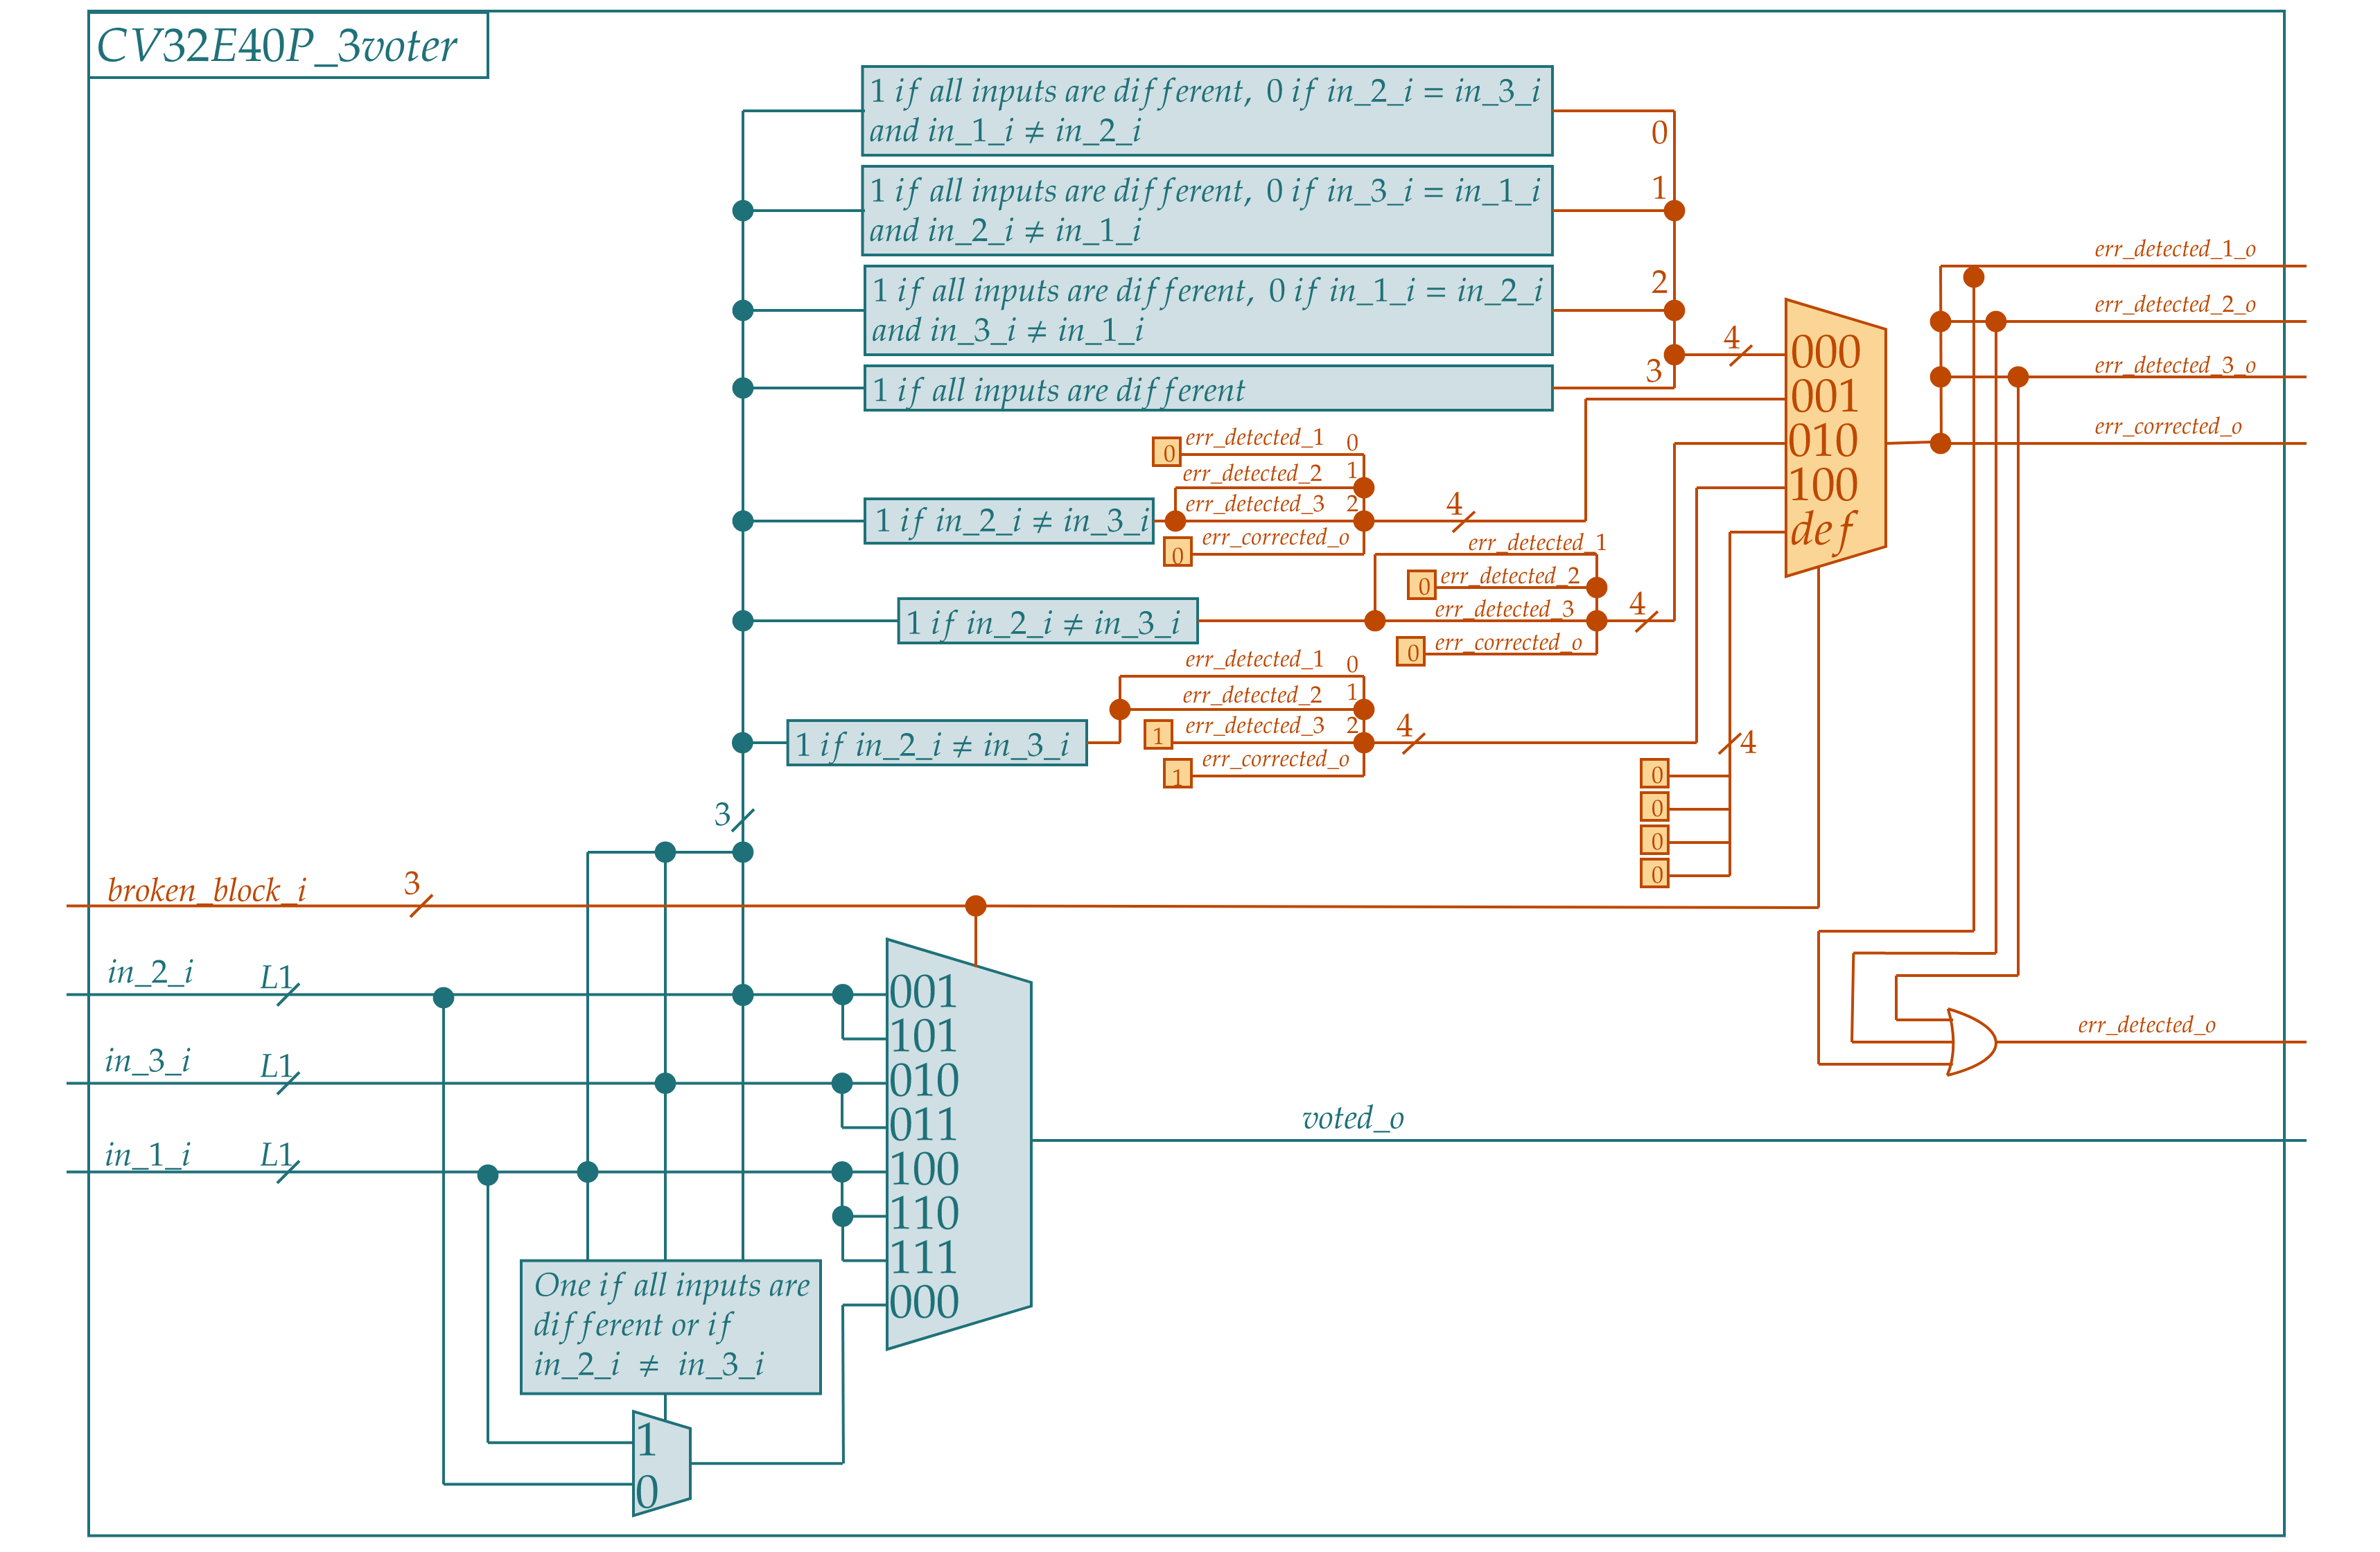
\includegraphics[width=1.1\textwidth,center]{./images/cv32e40p_3voter.png}
        		\caption{This is the voter used in the fault tolerant architecture.}
        		\label{fig:cv32e40p_voter}
        	\end{figure} 	
        	
        	The designed voter has also a three bit input called \textit{broken\_block\_i}, each bit refers to a block, zero means that the block works properly while 1 means that it has a permanent error.
            For example [0,0,0] means that all input signals come from blocks without permanent errors, instead [0,1,0] means that the second block have a permanent error.
            
            \textit{broken\_block\_i} allows the discarding of input signals from permanent faulty blocks.
            Indeed, the multiplexer on the left is controlled by the broken\_block\_i, e.g., when in\_1\_i comes from a permanent faulty block, in\_2\_i is automatically selected as output, so the system becomes a duplexer.\\
            
            In addition to the voting part there is some logic that indicates when there is a faulty input and when it is corrected by the voter.
            \textit{err\_detected\_1\_o}, \textit{err\_detected\_2\_o} and \textit{err\_detected\_3\_o} are one if the corresponding input signals in\_1\_i, in\_2\_i and in\_3\_i have a transient fault. When the input signal in\_x\_i is permanently faulty the corresponding output  err\_detected\_x\_o is zero, the remaining two output err\_detected\_y\_o and err\_detected\_z\_o will be both 1, if the corresponding inputs are different, because we can't know which is the correct input, otherwise they are zero.
            
           If the detected error has been corrected, the err\_corrected\_o signal is one, instead it is zero when all inputs are different.\\
            
            The cv32e40p\_3voter block can be used for single dimension array by changing the L1 parameter; this parameter changes the dimension of in\_x\_i and voted\_o signals, e.g.,if you have three 32-bit signals to compare, you have to set L1 to 32 to use the voter.\\
        
        }% cv32e40p\_3voter
        
        \subsection{Configurable Voter}{
            In order to enable triple voter configuration, we create the \textbf{cv32e40p\_conf\_voter}.
            This block can be used as a simple voter if TOUT is set to zero \figref{fig:cv32e40p_conf_voter}  or as a triple voter if TOUT is set to 1 \figref{fig:cv32e40p_conf_voter_tout1} .
            
            The external interface of the conf\_voter is equal to the cv32e40\_3voter apart for triple input called to\_vote\_i and triple output. 
            
            
            If TOUT is set to 0, the  output of the voter is connected to the first element of voted\_o, the other two elements aren't connected and they don't exist in the final layout.
            
            The three err\_detected signals of cv32e40\_3voter are grouped in block\_err\_o, so basically if TOUT is set to 0 the conf\_voter is approximately equal to the cv32e40p\_3voter.
            
            Instead if TOUT is set to 1, the conf\_voter creates three instances of cv32e40\_3voter and each voter votes independently the three inputs. The three outputs are connected to the voted\_o signal. 
            Finally the status signals are voted and sent to the output.
            
            As you can see, the external interface of the conf\_voter remains the same if you change TOUT, this allows a wide use of the block.\\
            
    	    \begin{figure}[H]
        		\centering
        		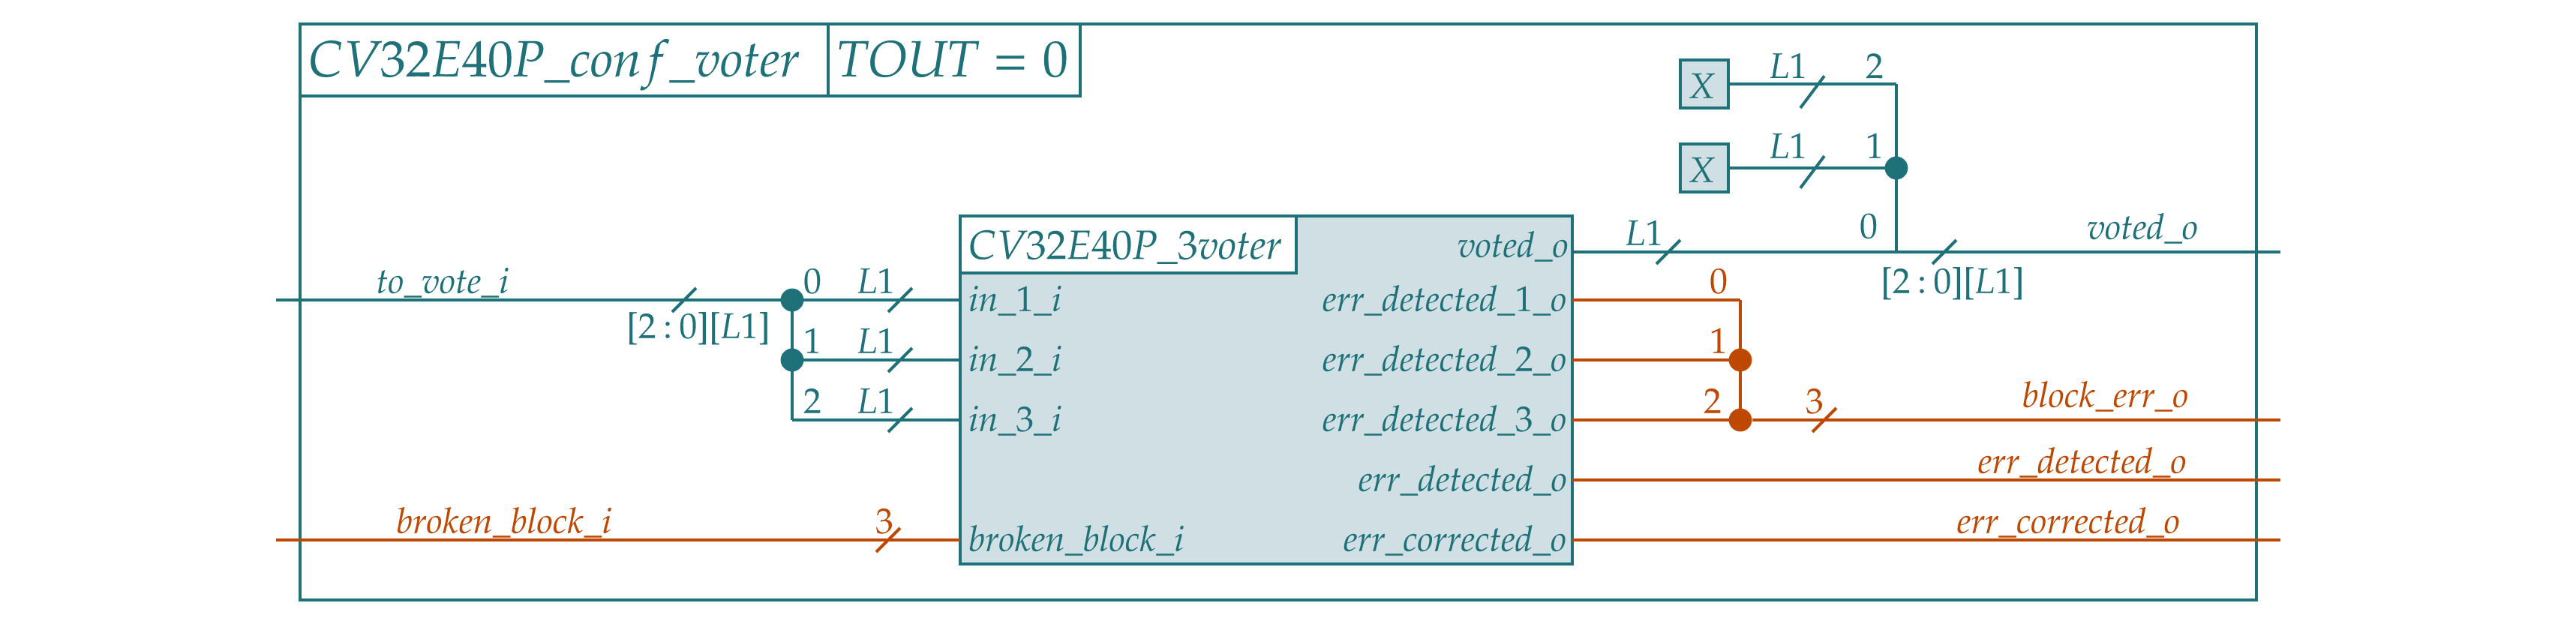
\includegraphics[width=1.3\textwidth,center]{./images/cv32e40p_conf_voter.png}
        		\caption{Configurable voter, with TOUT=0, a single voter.}
        		\label{fig:cv32e40p_conf_voter}
        	\end{figure} 	
        	
    	    \begin{figure}[H]
        		\centering
        		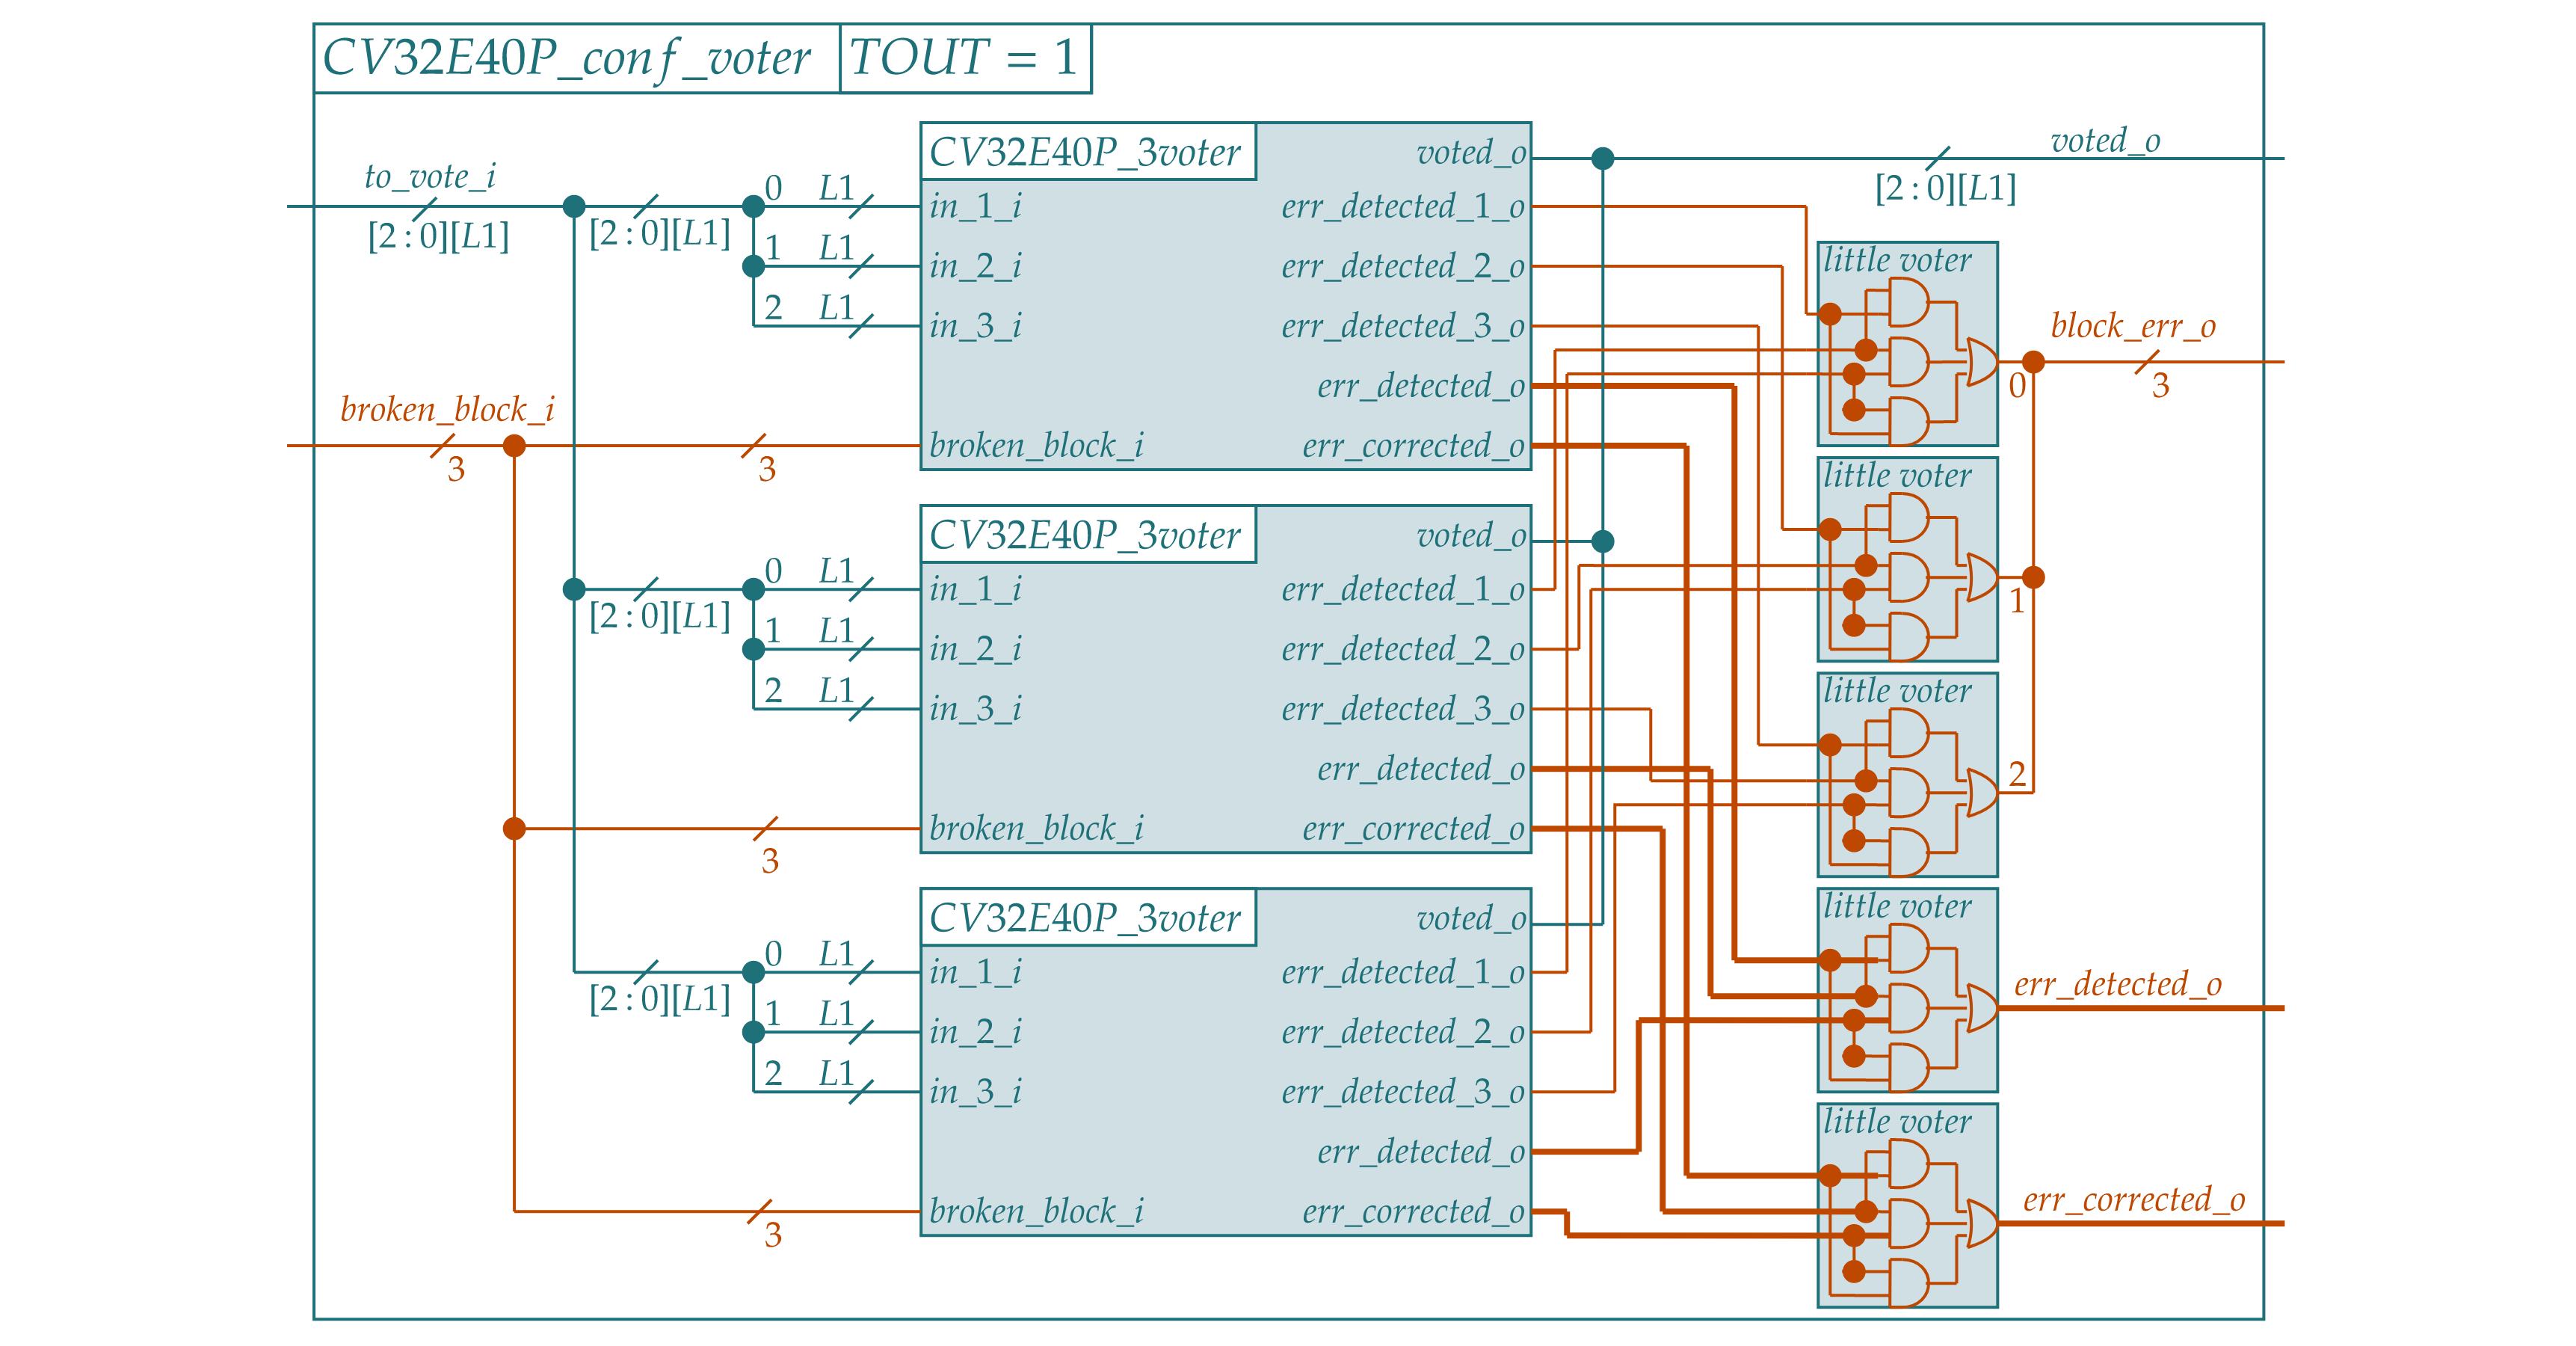
\includegraphics[width=1.3\textwidth,center]{./images/cv32e40p_conf_voter_tout1.png}
        		\caption{Configurable voter, with TOUT=1, a triple voter.}
        		\label{fig:cv32e40p_conf_voter_tout1}
        	\end{figure} 	
    	
    	}% end Configurable VOter
    	
    	\subsection{Breakage Monitor}{
    	    The third block is the \textbf{cv32e40p\_breakage\_monitor} in \figref{fig:cv32e40p_breakage_monitor}. 
    	    Each time the  Breakage Monitor is instanced we should associate it to one replica inside a NMR structure; in our case we have a TMR and so we will use three Breakage Monitor, one for each replica of the Compressed Decoder.
    	    Each time the associate block have an error, err\_detected\_i should be asserted. This error increases reg\_count\_q by an INCREMENT value.
    	    Instead, if err\_detected\_i is equal to zero reg\_count\_q is decreased by a DECREASE value; both INCREMENT and DECREASE are SV parameters that can be changed.
    	    When reg\_count\_q is higher than the  BREAKING\_THRESHOLD, is\_broken\_o is asserted, this causes the activation of the clock gating which freezes the block maintaining is\_broken\_o to one. The block can also be set broken using the set\_broken\_i input signal.\\
    	    
    	    This mechanism of increment and decrease allow to discard transient errors because their frequency is really low, so for one increment there are thousands of decreases. 
    	    Instead, when a permanent error exists, it typically appears more frequently and so the increase rate is higher, this leads to an increase of reg\_count\_q and, as a consequence, to the detection of a permanent error. 
    	    Anyway you can steer INCREMENT, DECREASE and BREAKING\_THRESHOLD parameters in order to fit the error rate of your application. 
    	    
    	    The SV module allows the change of the register size: INC\_DEC\_BIT is the number of bit for registers that contain INCREMENT and DECREASE variables, instead COUNT\_BIT is the number of bit of reg\_count register.
    	    Naturally we fit the number of bit with the parameter's values.\\
    	    
    	    \begin{figure}[H]
        		\centering
        		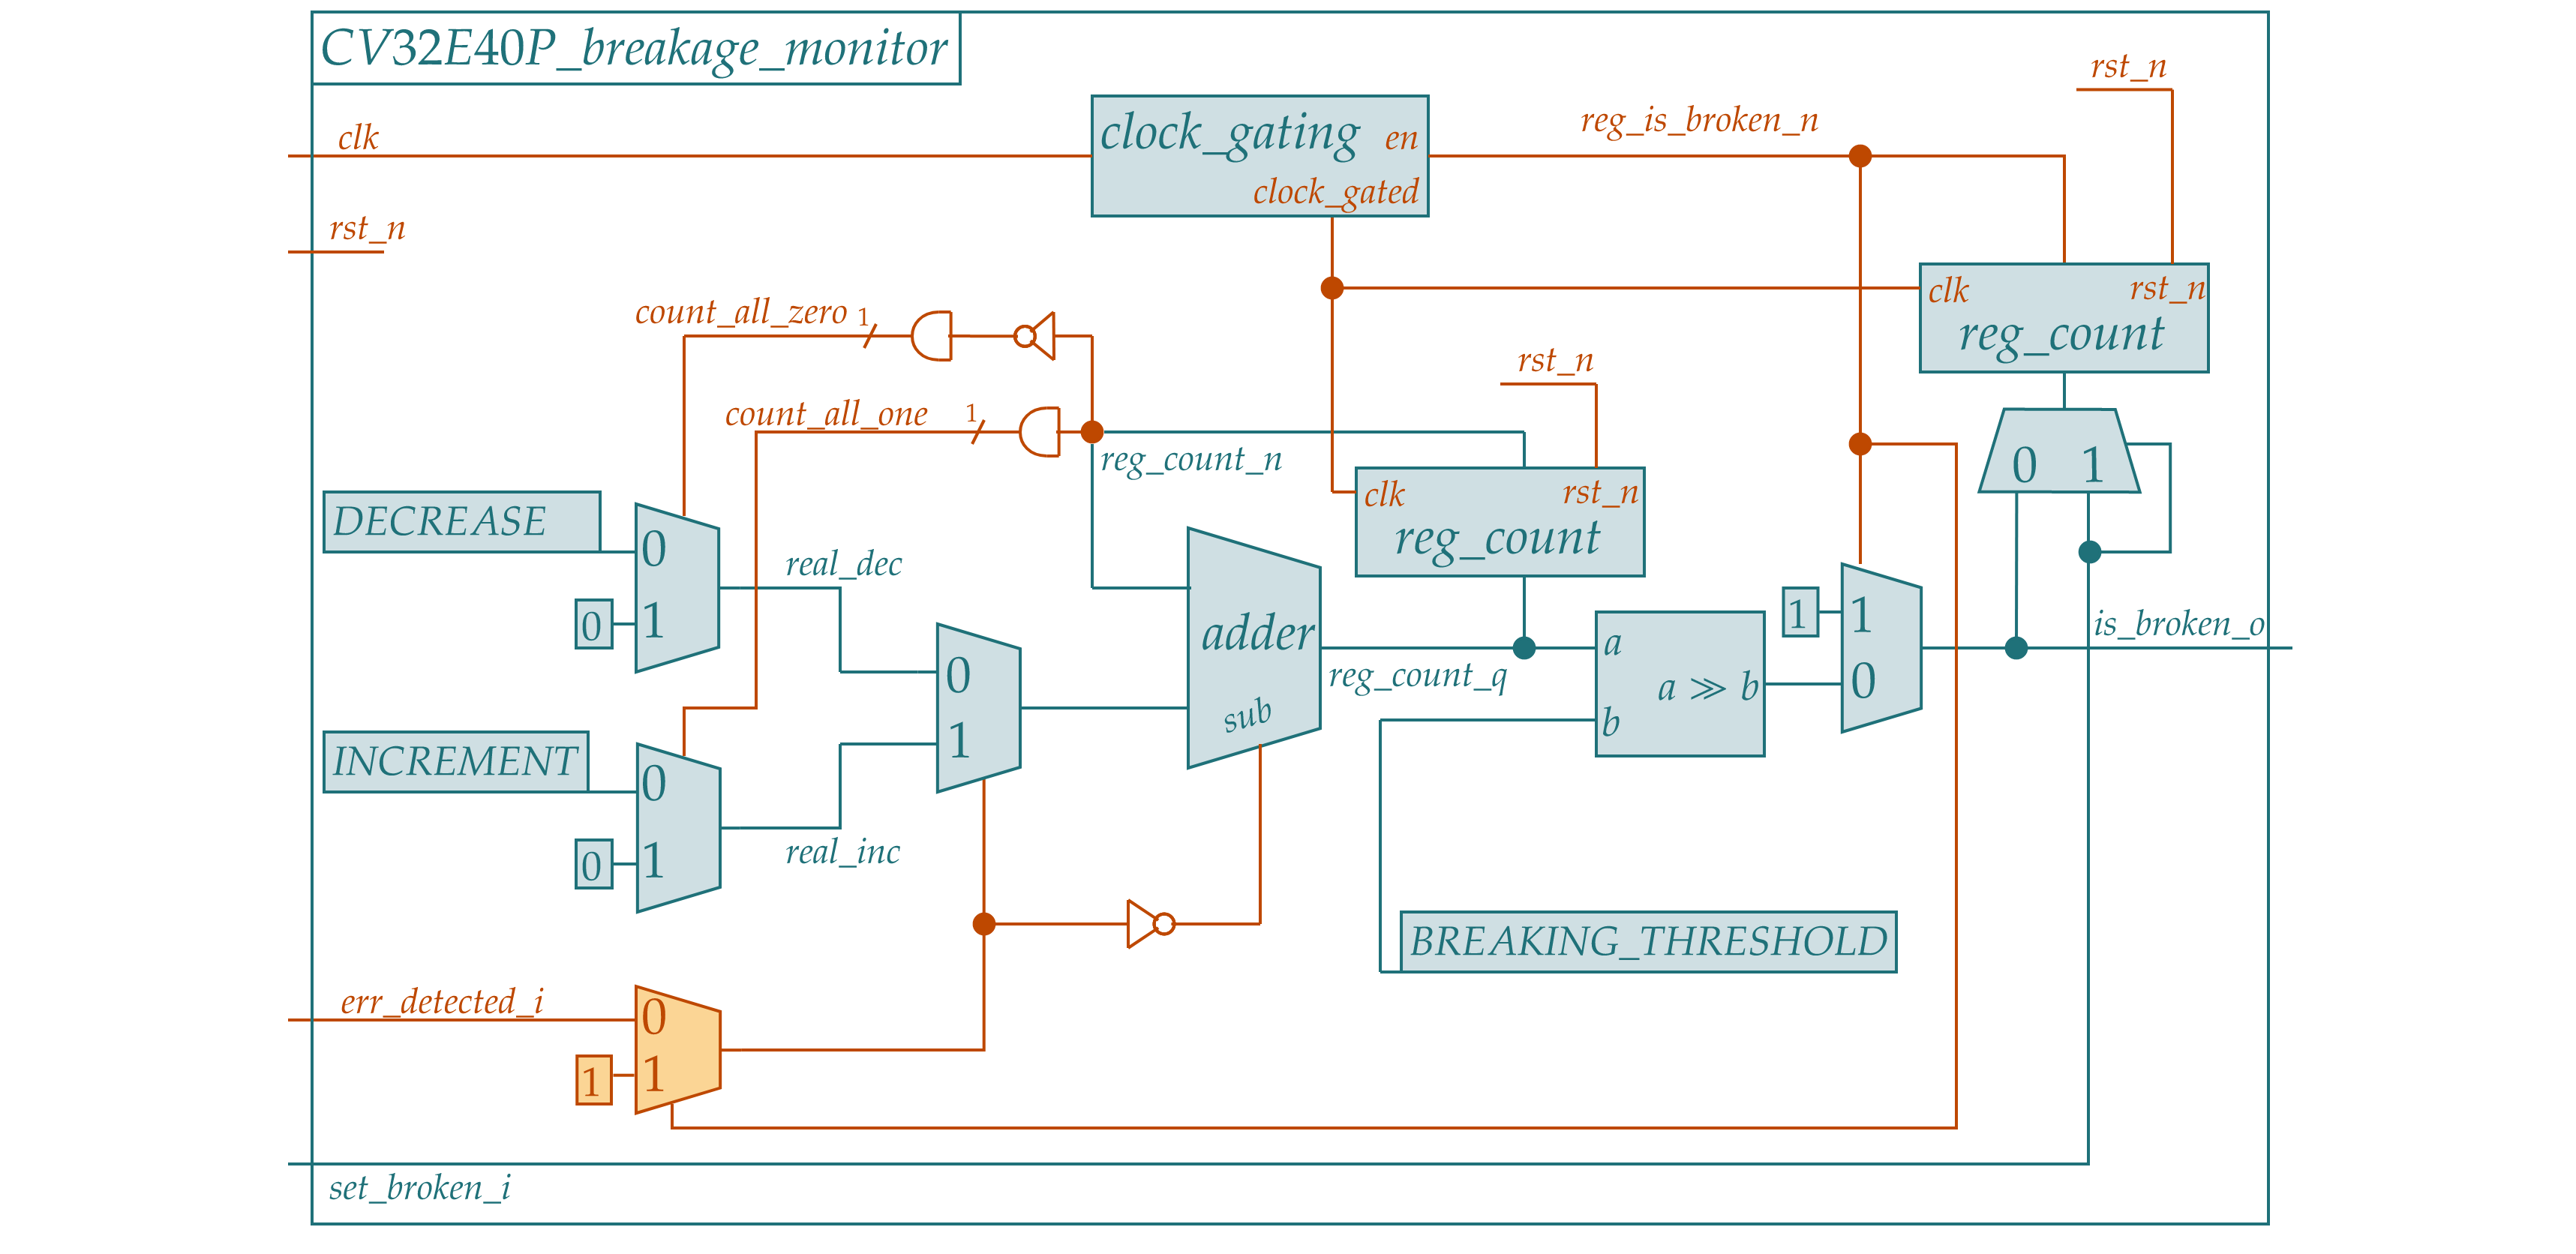
\includegraphics[width=1.3\textwidth,center]{./images/cv32e40p_breakage_monitor.png}
        		\caption{Breakage Monitor to detect permanent errors.}
        		\label{fig:cv32e40p_breakage_monitor}
        	\end{figure} 	
    	}% end Breakage Monitor	
    	\vspace{1cm}
    	
    	\subsection{Configurable Compressed Decoder}{
    	    \label{FTCD}
        	Finally we create the \textbf{cv32e40p\_compressed\_decoder\_ft} in \figref{fig:cv32e40p_compressed_decoder_ft}, using all previous blocks to create a new FT configurable Compressed Decoder (CD).
    		On the right there are three replicas of the CD, the nine outputs are grouped by name so all instr\_o outputs are connected to instr\_o\_to\_vote, is\_compressed\_o outputs are connected to is\_compressed\_o\_to\_vote and finally illegal\_instr\_o outputs are connected to illegal\_instr\_o\_to\_vote.
    		
    		These *\_to\_vote signals are connected to the relative conf\_voter, as you can see in \figref{fig:cv32e40p_compressed_decoder_ft} the first conf\_voter have three voter inside due to TOUT=1, this is an example of setting.\\
    	
    		Each conf\_voter have the block\_err\_o outputs, the first bit of these signals is referred to the errors of the first replica, the second bit to the second replica and the third to the third replica. The first block\_err\_o signal is referred to errors on instr\_o, the second block\_err\_o to is\_compressed\_o and the third to illegal\_instr\_o. 
    		
            We apply OR operation to each element of block\_err\_o in order to find possible errors in the corresponding replica, e.g., if the first replica have an error on is\_compressed\_o the second conf\_voter will have block\_err\_o=[1,0,0], while the other two conf\_voter will have block\_err\_o=[0,0,0], so we execute the OR between all block\_err\_o[0] and we find that is occured an error in the first replica.\\
            
            The outputs of the OR are connected to the inputs of the Breakage Monitor, in this way each Breakage Monitor controls the corresponding replica. 
            When a replica is considered broken by the Breakage Monitor the corresponding bit of the is\_broken\_o vector is set to 1 and all conf\_voter will no longer consider the corresponding block. 
            In this case the compressed\_decoder\_ft became a duplex system and if one of the two replicas failed the operation should be redone.\\
            
    		
    	    \begin{figure}[H]
        		\centering
        		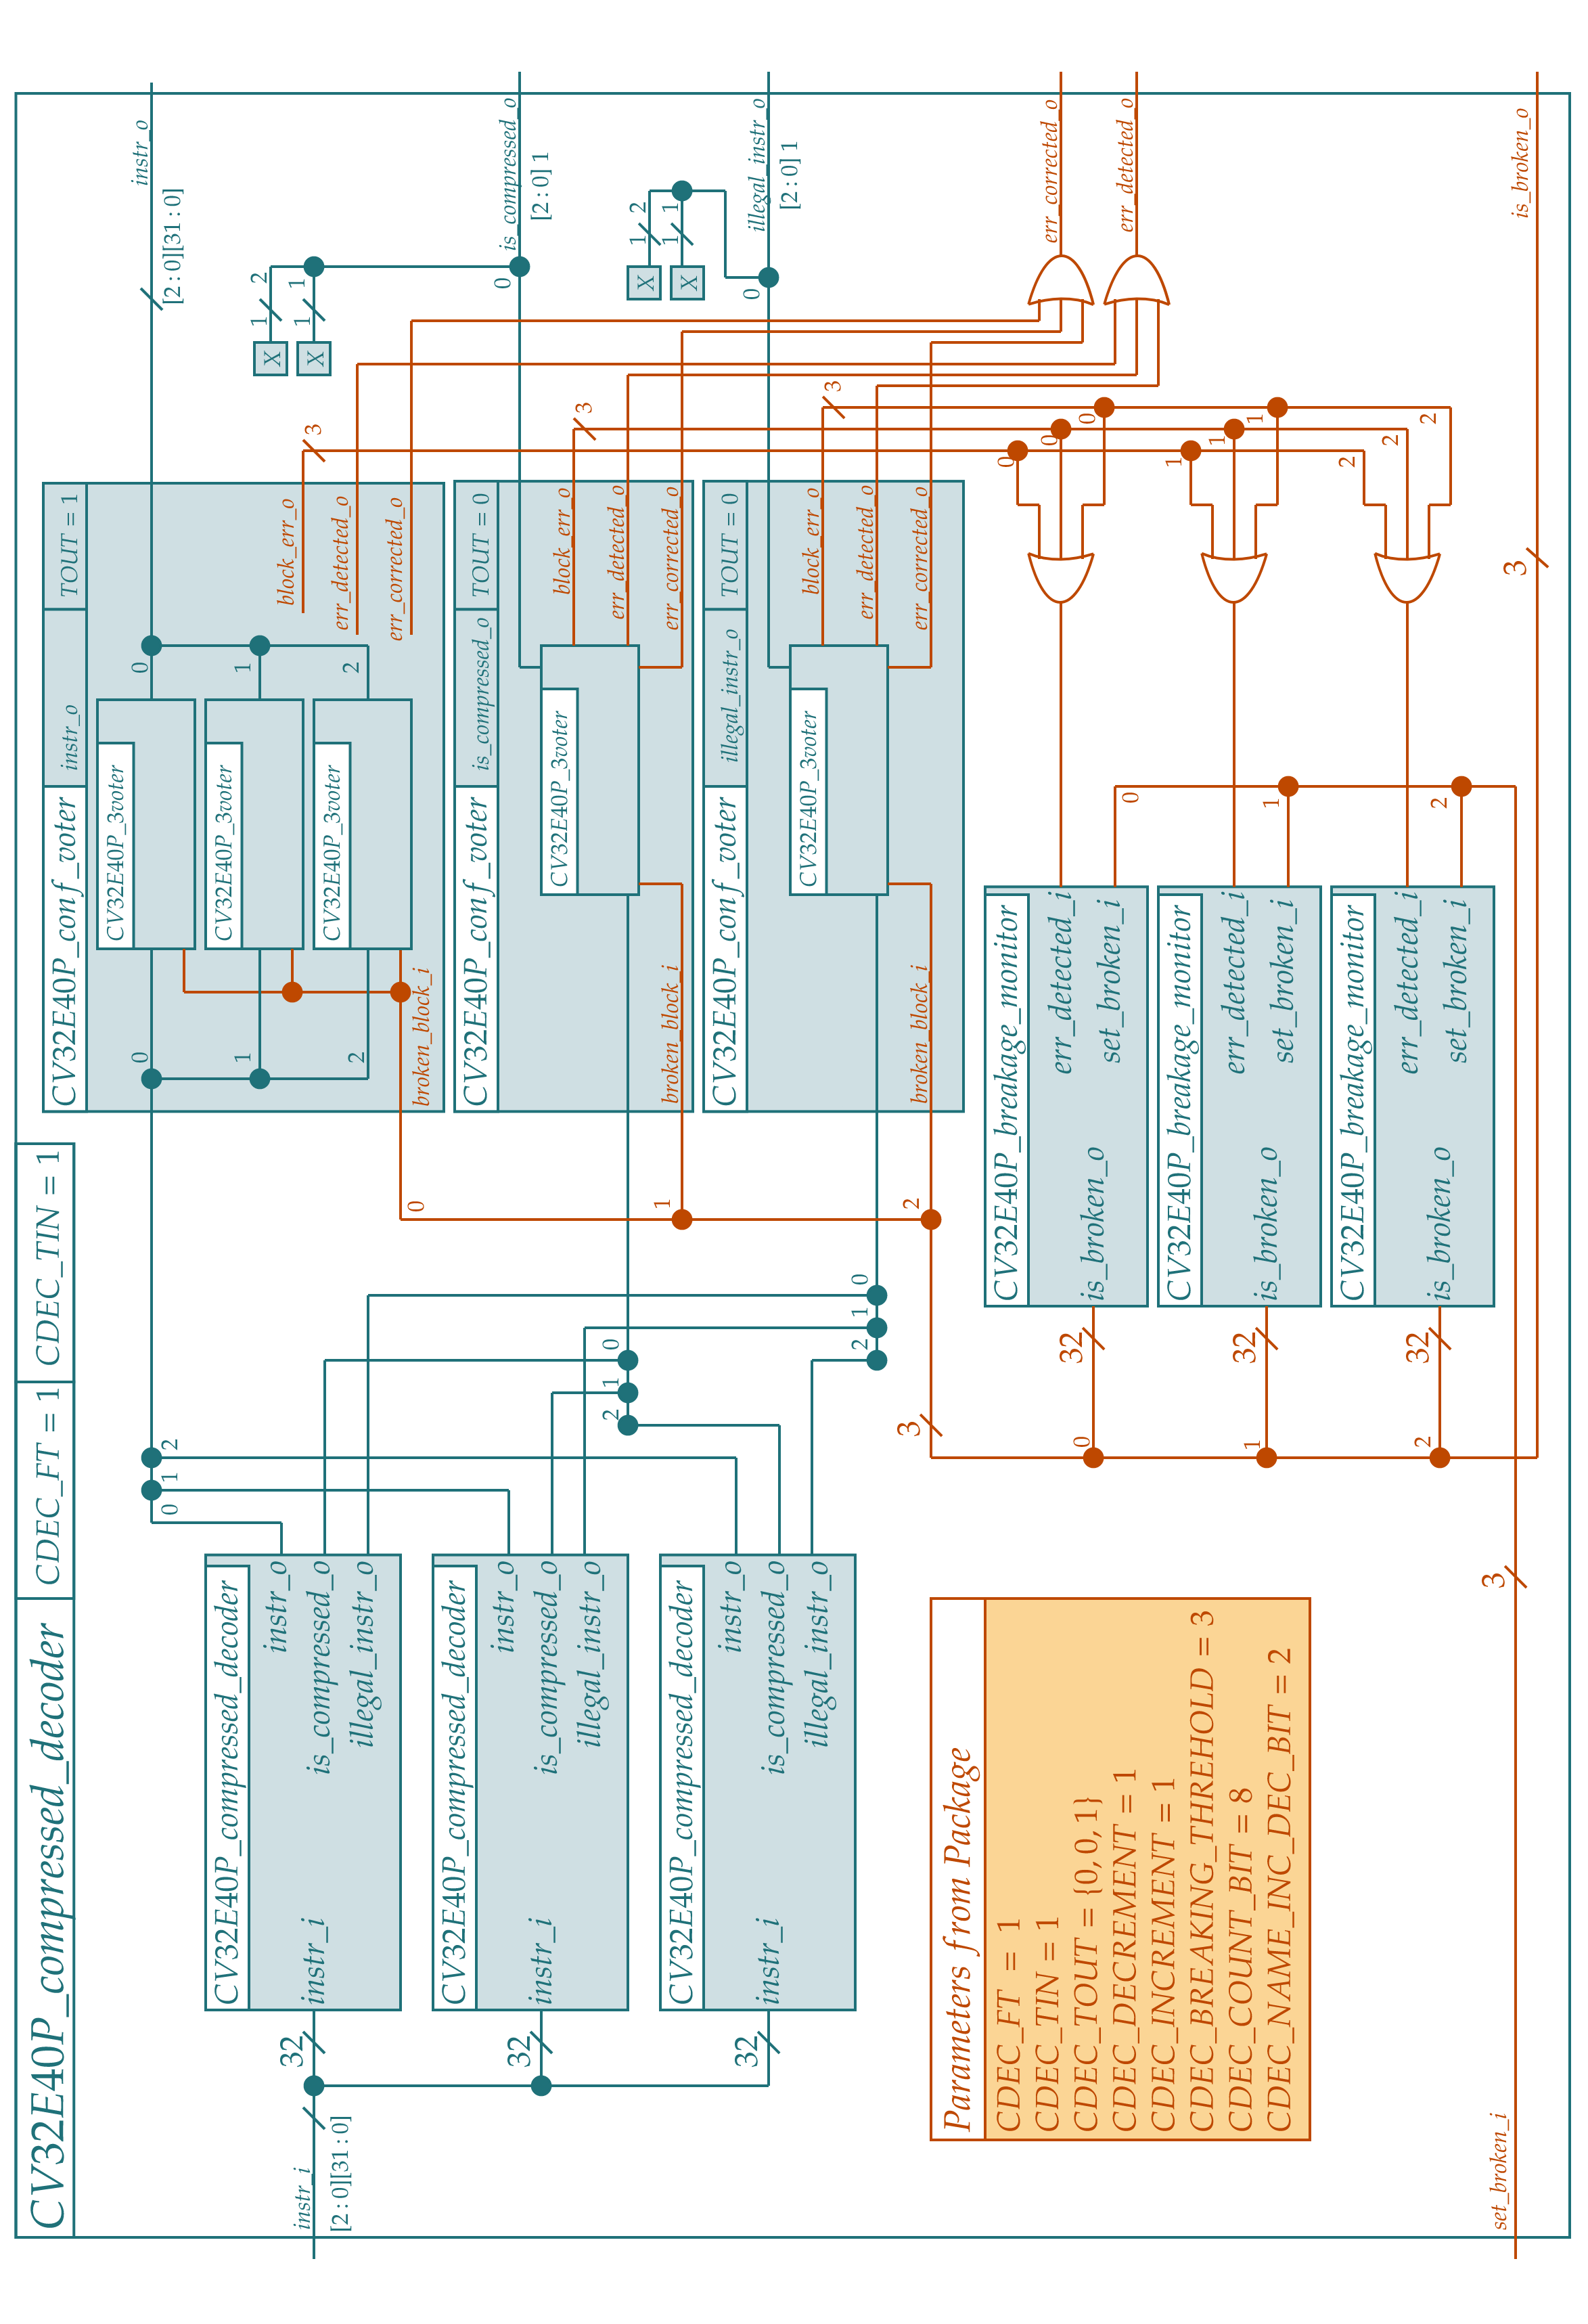
\includegraphics[width=0.95\textwidth,center]{./images/cv32e40p_compressed_decoder_ft.png}
        		\caption{A possible configuration of the Configurable Compressed Decoder.}
        		\label{fig:cv32e40p_compressed_decoder_ft}
        	\end{figure} 	
        	 
        	 set\_broken\_i is a three bit signal used to set broken a replica from outside the block, at the same time exist the is\_broken\_o signal used to communicate if there are permanent broken block to the outside of the block.
        	 
        	 The last signal can be used to save internal replicas status in some non-volatile memory ( e.g., CSR registers) and use these information to reload replicas status inside the FT compressed decoder if the system is rebooted with set\_broken\_i.\\
        	 
        	 
        	 Finally we have err\_corrected\_o and err\_detected\_o that communicate when an error occurs and if it has been corrected.
        	 These two signals can be used at high level to check architecture integrity and eventually indicate if the system should be replaced due to high error rate.\\
        	 
        	 In the Parameters From Package table there are all SV parameters that can be changed to configure the block. So the features of the block are:
        	 \begin{itemize}
        	     \item \textbf{Fault Tolerance:} If CDEC\_FT is equal to one is used TMR technique as you see in the picture, otherwise is used only one Compressed Decoder and the
        	     
        	     
        	     \breakline cv32e40p\_compressed\_decoder\_ft became the basic cv32e40p\_compressed\_decoder.
        	     \item \textbf{Triple Input:} When you set CDEC\_TIN is equal to one should be provided three instr\_i inputs, each input is connected to the corresponding compressed decoder, otherwise is used only one input equal for each replica. This feature is useful if the previous block implement triple voter configuration. 
        	     \item \textbf{Triple Output:} Each bit of CDEC\_TOUT corresponds to a conf\_voter and so to an output, the MSB is the last bit and it corresponds to the first output. The order of the output corresponds to the appearance order in the port declaration od the cv32e40p\_compressed\_decoder. When a bit of the CDEC\_TOUT is 1 the corresponding conf\_voter implement a triple voter, this means that the corresponding output will have three valid signals from triple voter.
        	     \item \textbf{Permanent Error Settings:} The remaining parameters are used to set the Breakage Monitor parameters, all Breakage monitor will have the same configuration.
        	 \end{itemize}
        	 
        	 As we have seen this block is highly configurable. 
        	 Due to triple input - output option both input and output signals are triplicated in the port declaration.
        	 Anyway in some configuration not all input and output signals are connected, this means that care must be taken in the block connection and parameters configuration.\\
        	 
        	 In the next chapter we will use the cv32e40p\_compressed\_decoder to create the Travulog template in order to automatically convert each sub-block of the IF stage.
         }% Configurable Compressed Decoder
    }% end FT Compressed Decoder
    
	\section{Travulog}{
	    \label{Travulog}
    	To create a configurable FT architecture it is necessary to apply fault tolerant techniques to all the blocks of the IF Stage and then allow to apply or not techniques in each block by means of parameters. It was therefore decided to create a metalanguage within the SystemVerilog (SV) that allows the creation of the new architecture starting from a template and a base module, in this way we can define a template and apply it to each block of the IF stage. The automatized application of Fault Fault tolerant methods already exists in some commercial application but it work at netlist level \bscite{SEU_effect_in_TMR_analytical}, our solution is at RTL level and it is open source. 
    	
    	As you can see in \figref{fig:TravulogFlowBlocks} the transformation of the main module is done by a Python object linked to the template, when you give the base module to the object a new module is created. The new FT architecture is created on the basis of the Travulog template and the base module, it is therefore an interface layer that makes the old module Fault Tolerant. 
    	To allow the conversion through the Travulog object it is necessary to have an object that contains all the data of the associated SystemVerilog base module, so we have created a new Python class that parses a SV file containing a module, this class has been called moddata. As shown in the \figref{fig:TravulogFlowBlocks} the file containing the basic module must be transformed into the corresponding moddata object and then passed to the Travulog object which generates the new architecture.
    	\begin{figure}[H]
    		\centering
    		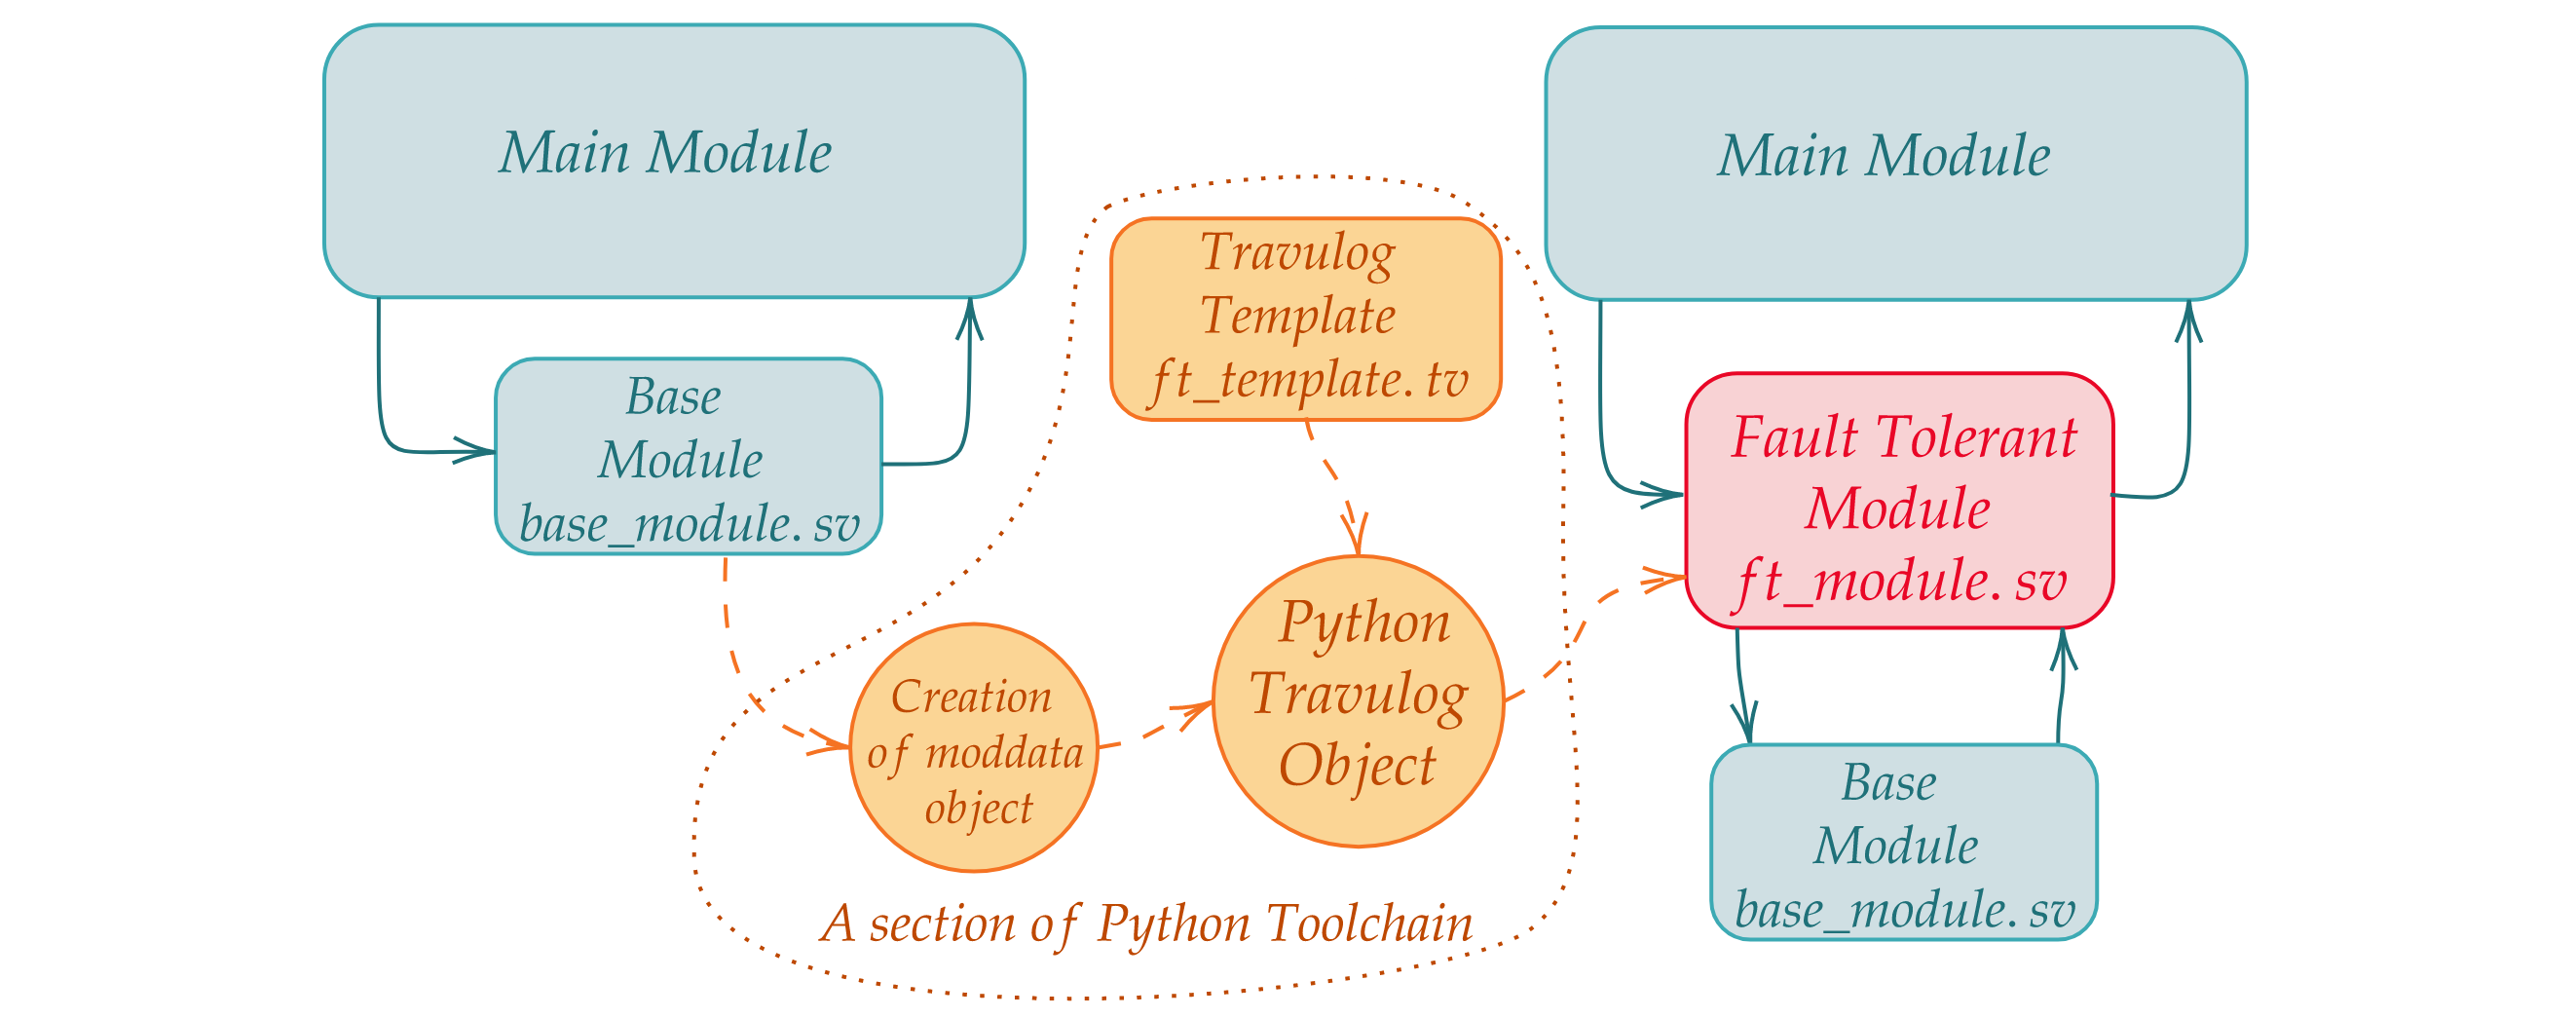
\includegraphics[scale=0.2,center]{./images/Travulog_flow_blocks.png}
    		\caption{Flow diagram of architecture transformation using Travulog template}
    		\label{fig:TravulogFlowBlocks}
    	\end{figure} 
    	
        The conversion of a SVerilog module using a Travulog template implies the use of Python code, in fact you have to create a moddata object related to the Base module, the Travulog object related to the TV template and then give moddata obj to TV obj to obtain the new SV code.	
        
        For these reason, in order simplify the use of Travulog template we create the Hidden Travulog (HTV) code or HTravulog. This code is hidden inside a synthesizable SV module using four slash and a space: "//// " . 
        
        This code should be written in the main SV module and it indicates how to apply Travulog template. Using HTV code you can also create new module from a SV block inside the current module and the apply your template to this new block. The complete functionality are described in HTravulog section. \\
	
	
    	To create the Travulog language we started from the fault tolerant 
    	compress\_decoder\_ft and we created a series of commands that allow us to create the FT compress decoder from the basic one. We will now analyze the various Travulog commands through pieces of the Travulog template and its conversion into SVerilog.
	
	
    	\subsection{Declaration of ports}{
    		Ports declaration is the first element in a System Verilog module, in this part of a new FT block probably you will see many of the IO signals of the basic architecture, for this reason we automatized the creation of this part allowing to use basic block signals name.\\
    		
    		In the listing \ref{lst:declTV} there is a part of the Travulog template, this piece of code allows to generate the System Verilog of the listing \ref{lst:declSV} which is the IO declaration of the FT Compressed Decoder. The Travulog commands used are the following : 
    		\begin{itemize}
    			\item [\textbf{PARAMETER\_DECLARATION}:] The command PARAMETER\_DECLARATION copies the parameter declaration from the BLOCK module in the new System Verilog module. BLOCK is an identifier used in the Travulog object that should be linked to a moddata object. Note that you can have multiple ID since they are managed as a diction:ary, e.g., if you set \{"BLOCK":moddata\_obj1, "BLOCK2":moddata\_obj2\} in the Travulog object you can use both BLOCK and BLOCK2 identifiers in the Travulog code.
    			\item [\textbf{DECLARATION\_FOREACH}:] This command cycles on the given signals and it substitutes: INOUT  with "input" or "output",  BITINIT with the bits definition and SIGNAME with the name of the signal. The first argument is the module id, the second one is the type of signal: IN for input port of the module, OUT for output, IN\_OUT for both input and output and INTERN for internal signals of the module. You can also indicate some signals to exclude from the list using "NOT sig1 sig2 ... " as you can see at line 7. e.g., clk and rst\_n signals are excluded since they should not be triplicated.
    			DECLARATION\_FOREACH can also be used for the declaration of internal signals and for assign statement as we will see later.
    			\item [\textbf{MODULE\_NAME}:] This is a parameter which is substituted with the name given to the Travulog object, it is the name of the new module.
    		\end{itemize}
    			
    			
    		\openup -0.5em
    		
    		\begin{parcolumns}[colwidths={1=0.54\textwidth}, distance=0.5em]{2}
    			\colchunk{%
    				\begin{lstlisting}[basicstyle=\ttfamily\scriptsize, language=Verilog, caption=Declaration Travulog Code, label=lst:declTV]
module MODULE_NAME
	
	PARAMETER_DECLARATION BLOCK

(
	// compressed decoder input output
	DECLARATION_FOREACH BLOCK IN_OUT NOT clk rst_n
		INOUT logic [2:0]BITINIT SIGNAME,
	END_DECLARATION_FOREACH

	
	input logic clk,
	input logic rst_n,  
	
	// fault tolerant state
	input logic [2:0] set_broken_i,
	output logic [2:0] is_broken_o,
	output logic err_detected_o,
	output logic err_corrected_o
);
    				\end{lstlisting}
    			}
    			\colchunk{%
    				\begin{lstlisting}[basicstyle=\ttfamily\scriptsize, language=Verilog, numbers=none, caption=Declaration SVerilog code derived, label=lst:declSV]
module cv32e40p_compressed_decoder_ft
#(
	parameter FPU = 0
)
(
	// compressed decoder input output
	input  logic [2:0] [31:0] instr_i,
	output logic [2:0] [31:0] instr_o,
	output logic [2:0] is_compressed_o,
	output logic [2:0] illegal_instr_o,
	
	input logic clk,
	input logic rst_n,    
	
	// fault tolerant state
	input logic [2:0] set_broken_i,
	output logic [2:0] is_broken_o,
	output logic err_detected_o,
	output logic err_corrected_o
);
    				\end{lstlisting}
    			}
    		\end{parcolumns}
    	
    		\openup +0.5em
    		
    		
    	}% end Declaration of ports
    	
    	\subsection{Internal signals and assign}{
    		In the following listings there is the continuation of the previous ports definition. The first "declaration\_foreach" create the signals used to connect the three block outputs to the voter while the second one creates block error signals. In the last two lines there is the compound parameter "SIG\_NUM-BLOCK-OUT" inside the square bracket,  this parameter is substituted in the right listing with the number (SIG\_NUM) of output ports (OUT) of the module (BLOCK) minus one, anyway instead of OUT you can use IN, PARAM, INTERN or IN\_OUT in order to have the correct signals number.
    		
    		\openup -0.5em
    		
    		\begin{parcolumns}[colwidths={1=0.5\textwidth}, distance=0.5em]{2}
    			\colchunk{%
    				\begin{lstlisting}[basicstyle=\ttfamily\scriptsize, language=Verilog, caption=Travulog Code, label=lst:internTV]
// Signals out to each compressed 
// decoder block to be voted
DECLARATION_FOREACH BLOCK OUT 
logic [2:0]BITINIT SIGNAME_to_vote ;
END_DECLARATION_FOREACH

// Error signals
DECLARATION_FOREACH BLOCK OUT 
logic [2:0] SIGNAME_block_err ; 
END_DECLARATION_FOREACH

// Signals that use error signal to 
// find if there is one error on each 
// block, it is the or of previous signals
logic [2:0] block_err_detected;
logic [SIG_NUM-BLOCK-OUT:0] err_detected;
logic [SIG_NUM-BLOCK-OUT:0] err_corrected;
    				\end{lstlisting}
    			}
    			\colchunk{%
    				\begin{lstlisting}[basicstyle=\ttfamily\scriptsize, language=Verilog, numbers=none, caption=SVerilog code derived, label=lst:internSV]
// Signals out to each compressed 
// decoder block to be voted
logic [2:0] [31:0] instr_o_to_vote ;
logic [2:0] is_compressed_o_to_vote ;
logic [2:0] illegal_instr_o_to_vote ;

// Error signals
logic [2:0] instr_o_block_err ;
logic [2:0] is_compressed_o_block_err ;
logic [2:0] illegal_instr_o_block_err ;

// Signals that use error signal to 
// find if there is one error on each 
// block, it is the or of previous signals
logic [2:0] block_err_detected;
logic [2:0] err_detected;
logic [2:0] err_corrected;
    				\end{lstlisting}
    			}	
    		\end{parcolumns}
    
    		\openup +0.5em
    	
    	} % end Internal signals and assign
    	
    	\subsection{Instance}{
    		\begin{comment}
    			Per poter creare una nuova instanza da un blocco esistente è stato creato il comando INSTANCE mostrato nel listing \ref{lst:instance1TV}. Dopo la keyword INSTANCE dev'essere indicato l'id del blocco e il nome della nuova instanza che verrà creata, come è mostrato nel listing seguente per creare il nome della nuova instanza viene utilizzato il parametro BLOCK_MODNAME, questo è sostituito in fase di preprocessamento con il nome del modulo a cui l'id BLOCK è riferito.
    			Successivamente all'interno del comando vengono indicate le connessioni da effettuare. PARAM si riferisce ai parametri e il comando a riga due indica di connettere i parametri allo stesso nome, infatti si ha .FPU(FPU). A riga 3 invece viene indicato di connettere i segnali clk e rst_n a stesso nome, la riga successiva connette gli ingressi al loro stesso nome ma aggiungendo il suffisso "[0]", dagli ingressi però vengono esclusi i segnali già connessi nell'if precedente. Nella conversione in SV che vedete sulla destra non sono presenti il clock e il reset quindi il comportamento indicato sopra non è evidente.
    			Come già accennato le connessioni all'interno del comando INSTANCE sono sensibili all'ordine in cui vengono fatte, percui per esempio gli IF sugli ingressi vanno fatti prima di assegnare genericamente gli ingressi con "IN = IN" altrimenti gli if non sono considerati. Stessa considerazione per le uscite e i parametri.
    		\end{comment}
    
            In order to create a new instance from an existing block, the INSTANCE command shown in the listing \ref{lst:instance1TV} was create. After the INSTANCE keyword, there are the block id and the name of the new instance. As shown in listing \ref{lst:instance1TV} the BLOCK\_MODNAME parameter is used to create the name of the new instance, this parameter is replaced in the preprocessing phase with the name of the BLOCK module.
            
            The connection commands are indicated inside the INSTANCE command. The command at line two indicates to connect the parameters to the same name, in fact we have .FPU (FPU). At line 3 instead it is indicated to connect clk and rst\_n signals to the same name, the next line connects the inputs to their same name but it adds the suffix "[0]", however, at the signals already connected in the previous if are not appended the suffix. In the conversion to SV on the right there are no clocks and no reset so the behavior just described is not evident.
            
            As already mentioned, the connections inside the INSTANCE command are sensitive to the order in which they are made, for example the IF on the inputs should be before assigning the inputs generically with "IN = IN", otherwise the ifs are not considered. Same consideration for outputs and parameters. 
        
    		\openup -0.5em
    	
    		\begin{parcolumns}[colwidths={1=0.5\textwidth}, distance=0.5em]{2}
    		\colchunk{%
    			\begin{lstlisting}[basicstyle=\ttfamily\scriptsize, language=Verilog, caption=Instance Travulog Code, label=lst:instance1TV]
INSTANCE BLOCK BLOCK_MODNAME_no_ft
PARAM=PARAM
IF clk rst_n IN=IN
IN= IN[0]
OUT = OUT[0]
END_INSTANCE
    
    
    
    
    
    	
    	
    	
    	
    	
    			\end{lstlisting}
    		}
    		\colchunk{%
    			\begin{lstlisting}[basicstyle=\ttfamily\scriptsize, language=Verilog, numbers=none, caption=Instance SVerilog code derived, label=lst:instance1SV]
cv32e40p_compressed_decoder
#(
    .FPU (FPU)
)
compressed_decoder_no_ft
(
    // Input ports of compressed_decoder_no_ft
    .instr_i                (  instr_i[0]),

    // Output ports of compressed_decoder_no_ft
    .instr_o        (  instr_o[0]),
    .is_compressed_o(  is_compressed_o[0] ),
    .illegal_instr_o(  illegal_instr_o[0] )
);		
    			\end{lstlisting}
    		}	
    		\end{parcolumns}
    	
    		\openup +0.5em
    		
        	
        	In the cv32e40p\_compressed\_decoder\_ft module there are as many conf\_voter as the output of the cv32e40p\_compressed\_decoder (CD), in fact the CD is triplicated and we need a conf\_voter for each output. In order to automatize the creation and the connection of the conf\_voter we create the command INSTANCE\_FOREACH. After this keyword there is the id of the block and the list of signals on which cycle on. It can be used IN, OUT, IN\_OUT and INTERN as abbreviation for the list, in this way the code is compressed and clearer.
        	
        	
        	As just mentioned INSTANCE\_FOREACH cycles on the signals list and it substitutes in the verilog code: BITNUMBER with the number of bits of the signal, INDEX with the current cycle number and SIGNAME with the name of the signal.
        
        	In the listing below you can see an example of how the INSTANCE\_FOREACH command works.
        	
    		\openup -0.5em
    	
    		\begin{parcolumns}[colwidths={1=0.5\textwidth}, distance=0.5em]{2}
    		\colchunk{%
    			\begin{lstlisting}[basicstyle=\ttfamily\scriptsize, language=Verilog, caption=Instance  foreach  Travulog  Code, label=lst:instance2TV]
INSTANCE_FOREACH BLOCK OUT    
    // Voter for TOVOTE signal, triple voter if
    // PARAM_NAME_TOUT[INDEX] == 1
    cv32e40p_conf_voter
    #(
        .L1(BITNUMBER),
        .TOUT(PARAM_NAME_TOUT[INDEX])
    ) voter_SIGNAME_INDEX
    (
        .to_vote_i( SIGNAME_to_vote ),
        .voted_o( SIGNAME),
        .block_err_o( SIGNAME_block_err),
        .broken_block_i(is_broken_o),
        .err_detected_o(err_detected[INDEX]),
       .err_corrected_o(err_corrected[INDEX])
    );
END_INSTANCE_FOREACH
    
    
    
    
    
    
    
    
    
    
    
    
    
    
    
    
    
    
    
    
    
    
    
    
    
    
    
    
    
    			\end{lstlisting}
    		}
    		\colchunk{%
    		    \begin{lstlisting}[basicstyle=\ttfamily\scriptsize, language=Verilog, numbers=none, caption=Instance foreach SVerilog code , label=lst:instance2SV]
// Voter for TOVOTE signal, triple voter if
 // CODE_TOUT[0] == 1
cv32e40p_conf_voter
#(
    .L1(32),
    .TOUT(CODE_TOUT[0])
) voter_instr_o_0
(
    .to_vote_i( instr_o_to_vote ),
    .voted_o( instr_o),
    .block_err_o( instr_o_block_err),
    .broken_block_i(is_broken_o),
    .err_detected_o(err_detected[0]),
    .err_corrected_o(err_corrected[0])
);
// Voter for TOVOTE signal, triple voter if
// CODE_TOUT[1] == 1
cv32e40p_conf_voter
#(
    .L1(1),
    .TOUT(CODE_TOUT[1])
) voter_is_compressed_o_1
(
    .to_vote_i( is_compressed_o_to_vote ),
    .voted_o( is_compressed_o),
    .block_err_o( is_compressed_o_block_err),
    .broken_block_i(is_broken_o),
    .err_detected_o(err_detected[1]),
    .err_corrected_o(err_corrected[1])
);
// Voter for TOVOTE signal, triple voter if
// CODE_TOUT[2] == 1
cv32e40p_conf_voter
#(
    .L1(1),
    .TOUT(CODE_TOUT[2])
) voter_illegal_instr_o_2
(
    .to_vote_i( illegal_instr_o_to_vote ),
    .voted_o( illegal_instr_o),
    .block_err_o( illegal_instr_o_block_err),
    .broken_block_i(is_broken_o),
    .err_detected_o(err_detected[2]),
    .err_corrected_o(err_corrected[2])
);
    			\end{lstlisting}
    		}	
    		\end{parcolumns}
    	
    		\openup +0.5em
    		
    	} % end instance
    
    	\subsection{Multiple Operation}{
            An instance of compressed\_decoder have an error if there is at least one output signal wrong, for these reason error\_detected signals is found by applying OR operation between *\_block\_err signals out of the conf\_voters as explained in Section \ref{FTCD}. The number of *\_block\_err signals is equal to the number of output of the module used, in this case the three output of the compressed\_decoder, for this reason we create the Travulog command OP\_FOREACH that apply a logic operation to a set of signals. 
            
            After the keyword OP\_FOREACH there should be the module id and then the signals identifier (IN, OUT, IN\_OUT, INTERN, PARAM), these two element identify the list of signals to cycle on. Then there should be the operation to apply ( |, \& etc ) and the pattern to use for each signal ( SIGNAME will be replaced with the name of the signal).
            
            In the listing \ref{lst:multiopTV} is applied a  suffix to the signame in order to apply OR to correct block\_err signals, instead in the right listing there is the conversion of Travulog code, each TV line becomes three lines of SV. 
    	
    		\openup -0.5em
    	
    		\begin{parcolumns}[colwidths={1=0.5\textwidth}, distance=0.5em]{2}
    		\colchunk{%
    			\begin{lstlisting}[basicstyle=\ttfamily\scriptsize, language=Verilog, caption=Instance  foreach  Travulog  Code, label=lst:multiopTV]
assign block_err_detected[0] = OP_FOREACH BLOCK OUT | SIGNAME_block_err[0] ; 


assign block_err_detected[1] = OP_FOREACH BLOCK OUT | SIGNAME_block_err[1] ; 


assign block_err_detected[2] = OP_FOREACH BLOCK OUT | SIGNAME_block_err[2] ; 



        		\end{lstlisting}
    		}
    		\colchunk{%
    		    \begin{lstlisting}[basicstyle=\ttfamily\scriptsize, language=Verilog, numbers=none, caption=Instance foreach SVerilog code , label=lst:multiopSV]
assign block_err_detected[0] =  
          instr_o_block_err[0]
        | is_compressed_o_block_err[0]
        | illegal_instr_o_block_err[0]; 
assign block_err_detected[1] =  
          instr_o_block_err[1]
        | is_compressed_o_block_err[1]
        | illegal_instr_o_block_err[1]; 
assign block_err_detected[2] =  
          instr_o_block_err[2]
        | is_compressed_o_block_err[2]
        | illegal_instr_o_block_err[2]; 

    			\end{lstlisting}
    		}	
    		\end{parcolumns}
	
    		\openup +0.5em
        	
    	}% end Multiple Operation 
    	
    	\subsection{Converted SV and parameters template}{
            At the end of the Travulog conversion you will obtain the compressed\_decoder\_ft.sv file (listing \ref{lst:cdftSV} ) containing an architecture layer that makes the compressed\_decoder fault tolerant.
            
    		\openup -0.5em
    	
        	\lstinputlisting[basicstyle=\ttfamily\scriptsize, language=Verilog, caption=Fault Tolerant compressed decoder layer, label=lst:cdftSV]{./code/cv32e40p_compressed_decoder_ft.sv}
        	
    		\openup +0.5em
    		
    		This SVerilog architecture needs some parameters: CODE\_FT, CODE\_TIN,
    		
    		CODE\_TOUT,  CODE\_DECREMENT,  CODE\_INCREMENT,     
    		
    		CODE\_BREAKING\_THRESHOLD,     
    		CODE\_COUNT\_BIT, CODE\_INC\_DEC\_BIT. 
    		
    		These parameters are contained in the cv32e40p\_pkg2 package imported at line one of listing \ref{lst:cdftSV}, the creation of this package can be automatized using a TV parameters template, for example our fault tolerant TV template ft\_template.sv needs its TV parameters template ft\_template\_parameters.sv, this template is shown in listing \ref{lst:paramTV}.
    		
    		
    		\openup -0.5em
    	
        	\lstinputlisting[basicstyle=\ttfamily\scriptsize, language=Verilog, caption=Parameters template for Fault tolerant module, label=lst:paramTV]{./code/ft_template_parameters.sv}
        	
    		\openup +0.5em
    		
    		This Template should be converted in System Verilog using our Toolchain.
    		
    		
    	}% end parameters template
    	
    	\subsection{Apply the template in Python}{
            In order to apply the Travulog template to a module you can use HTravulog code where the module is instanced or you can directly use Python code. In this section we follow the second way and so we explain how Python code is structured and how to use it.
            
            The whole code of the toolchain is in the \url{https://github.com/Elia1996/Travulog} repository, so you can clone it and use it. 
            
            In order to use Travulog template you need the files \textit{moddata.py} and \textit{travulog.py}, the first file contains many functions and the moddata class that enable the parsing an manipulation of a SVerilog module, instead the second file contains the travulog class.
            
            If you want to apply a Travulog template, the faster way is to look at test\_travulog.py file reported below.
            \begin{lstlisting}[basicstyle=\ttfamily\scriptsize, language=Python, caption=Basic Python code to use Travulog, label=lst:texttravulog]
#!/usr/bin/python3
from travulog import *

template_fname = "templates/ft_template.sv"
template_params_fname = "templates/ft_template_parameters.sv"
module_fname_dict = {"BLOCK" : "./test/arch/cv32e40p_compressed_decoder.sv"}
module_prefix = "cv32e40p_"

tr = travulog(template_fname, template_params_fname, module_fname_dict, module_prefix)

print(tr.GetElaboratedTemplate("New_module_name","PARAM_NAME"))
print(tr.GetElaboratedTemplateParams("New_module_name","PARAM_NAME"))
            \end{lstlisting}
            
            As you can see after the import of the travulog module are defined some parameters: 
            \begin{itemize}
                \item \textbf{template\_fname:} this is the fault tolerant template written in Travulog, the extension is irrelevant.
                \item \textbf{template\_params\_fname:} this is the TV template of parameters, it is used at line twelve where it is converted according to the current module name that in our case is the compressed\_decoder,
                \item \textbf{module\_fname\_dict:} This is a dictionary which connects modules ids with corresponding filenames of SVerilog modules. In this case BLOCK is connected to the compressed\_decoder filename and for this reason the Travulog object create the fault tolerant compressed decoder. Anyway you can have multiple module ids inside the TV template, you only need to set it in this dictionary.
                \item \textbf{module\_prefix:} This should be the prefix of each filename and module name, it should always end with a  "\_" character and it is used to create correct parameter base name.
            \end{itemize} 
            
            Once created the travulog object using these parameters, you can use GetElaboratedTemplate function to create the new cv32e40p\_compressed\_decoder\_ft.sv file text and you can use GetElaboratedTemplateParams function to create the parameters initialization for the package.
            For directly use the new architecture you should create a new package file containing the parameters initialization and import this package in the new ft module.
        
        }
    
    The way in which has been structured the Python code enable the creation of new powerful Travulog commands, so the TV commands analyzed is only a small example of what can be done using this tool since TV code can be extended according to your architectural needs. 
	}% end RISCV 32bit ISA 

    \newpage
	\section{Hidden Travulog}{
	    \label{HTravulog}
        As already mentioned, Hidden Travulog or HTV is a particular comment code inside a SVerilog file, the difference respect to a comment is the "//// " beginning key (HTKEY) instead of "//". The HTV parser only analyze the code after the HTKEY so be careful to correcty write "//// " before the HTV code.
        
        The result of a hidden code as HTV is the higher architecture maintenance, indeed the SVerilog architecture can be simulated, synthesised and modified with HTV code in it. After that a change in the base arch is done you can proceed with the HTravulog conversion, at the end of the process you obtain a new architecture that contains the base architecture changes. This maintenance process is shown in figure \ref{fig:HtravulogCycle}.
		\begin{figure}[H]
			\centering
			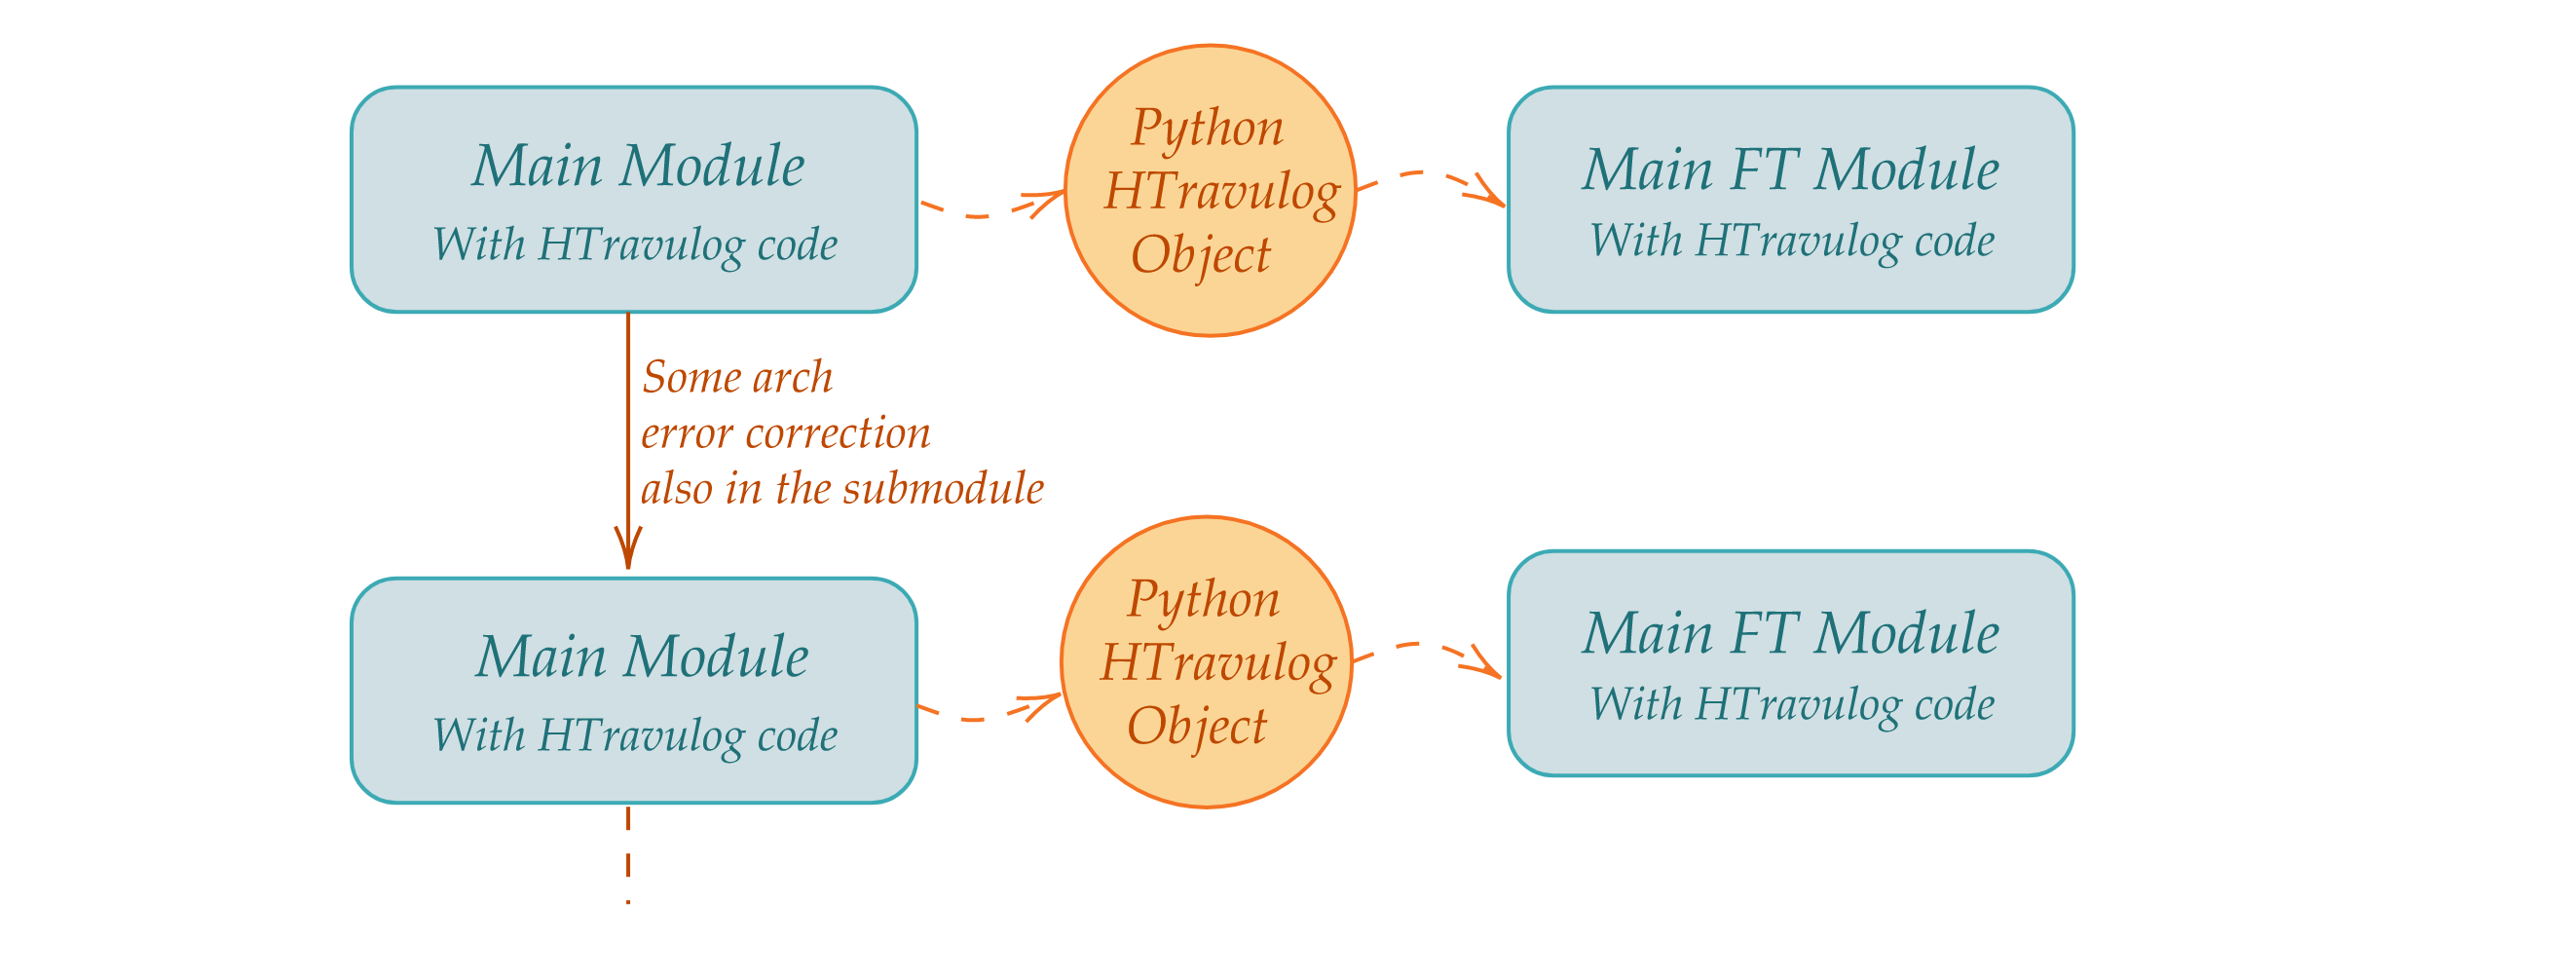
\includegraphics[scale=0.2,center]{./images/HTravulogArchMaintenance.png}
			\caption{HTravulog used during architecture life cycle}
			\label{fig:HtravulogCycle}
		\end{figure} 
        
        For the purpose of this Master Thesis are created only few HTV commands that can be extended for other uses. Anyway at this implementation step, HTV code can be used inside a whatever SVerilog module for these purpose:
        \begin{itemize}
            \item \textbf{Add some line:} The command ADD\_LINE allows to add an arbitrary line to the converted architecture.
            \item \textbf{Change internal signals:} The command FOREACH allows to cycle on input, output, internal signals and parameters in order to use their name for some connections or declarations.
            \item \textbf{Create new module:} When you want to apply a Travulog template to a piece of your \textit{architecture called A} but it is written as a part of the module, you can use CREATE\_MODULE command. With this command you can transform the piece of \textit{arch A} in a new \textit{module B} written in a new SV file, additionally the command automatically creates the instance of \textit{module B} in the converted \textit{architecture A}. 

            \item \textbf{Apply a Travulog template to a module:} In the main module of an architecture you normally have many instances of modules, for each instance you can use ADD\_MODULE\_LAYER. This commmand transforms the instanced module using a Travulog template and it create the new correct instance.
        \end{itemize}
        
        These are the main transformation you can apply with HTravulog code.
        
        Now in order to explain how HTV parser works we divide SVerilog module in these four parts:
        
        \begin{itemize}
            \item \textbf{Introduction:} It is the SV code from the beginning of the file up to the module declaration, here you usually import package and you write the architecture license. In this part you can use these HTV commands: IMPORT, ADD\_LINE, NEW\_MODULE\_NAME and  NEW\_MODULE\_FILE. These command are explained in \ref{Introduction} section.
            
            \item \textbf{Port declarations:} In this part are defined the input and output of the module, at the moment this part can't be modified in order to maintain the same interface, anyway the code is organized in order to simplify the extension of HTV code also in this part.
            
            \item \textbf{Intern signals and assign:} This part starts at the end of port declaration and ends with the HTV command "END\_DECLARATIONS", In this part you should define all intern signals and all assignment that you want to change during conversion. Just before the begin of the architecture structure definition you should place the "END\_DECLARATIONS" command in order to notify the tool that the third part ends. This part is analyzed in Section \ref{InternalSignals}.
            
            In this section you can use only the command FOREACH.
            
            \item \textbf{Architecture definition:} This part starts after the  "END\_DECLARATIONS" command and ends with the module. Here you can use CREATE\_MODULE and ADD\_MODULE\_LAYER commands, these are two powerful commands that are described in section \ref{CreateNewModule} and \ref{AddModuleLayer}.
            
        \end{itemize}
        
        In the following section we analyze each part and each command in detail.
        
        \subsection{Introduction Part}{
            \label{Introduction}
            This is the part of code before the declaration of the module, in listing \ref{lst:ifstageIntro} there is an example of SV mixed with HTV code used in cv32e40p\_if\_stage.sv
            file.
            
            
            \begin{lstlisting}[basicstyle=\ttfamily\scriptsize, language=Verilog, caption=Introduction of cv32e40p if stage, label=lst:ifstageIntro]
//// IMPORT htv_pkg.tv

import cv32e40p_pkg::*;
//// ADD_LINE import cv32e40p_pkg2::*;

//// NEW_MODULE_NAME cv32e40p_if_stage
//// NEW_MODULE_FILE OUT_DIR/cv32e40p_if_stage_ft.sv
            \end{lstlisting}
            
            \paragraph{IMPORT command:}{
                \label{par:import}
                At line one there is the IMPORT command used to import a parameters file, this file is parsed by the tool in order to import some parameters. In listing \ref{lst:htvpkg} there is an example of \textit{htv\_pkg.tv} file, all parameter are mandatory. BASEDIR is an abbreviations of the complete base path, we use BASEDIR for space reasons but the real file contains the complete path. 
                
                \begin{lstlisting}[basicstyle=\ttfamily\scriptsize, language=Verilog, caption=Introduction of cv32e40p if stage, label=lst:htvpkg]
IN_DIR BASEDIR/test/arch
OUT_DIR BASEDIR/out
TEMPLATE ft_template
        FILE BASEDIR/templates/ft_template.sv
        PARAM_FILE BASEDIR/templates/ft_template_parameters.sv
END_TEMPLATE
PKG_FILE BASEDIR/templates/cv32e40p_pkg2.sv
PKG_OUT_FILE BASEDIR/out/cv32e40p_pkg2.sv
MODULE_PREFIX cv32e40p_
                \end{lstlisting}
                
                The first two line set IN\_DIR and OUT\_DIR, these two parameters can be used in the main file as abbreviations of the corresponding directory set. Usually you set IN\_DIR as the directory where there is all base architecture and OUT\_DIR as the directory where you want to save the transformed architecture.
                
                The TEMPLATE statement is a command that you should use to define Travulog templates used in ADD\_MODULE\_LAYER command as you can see in listing \ref{lst:htvpkg2}. Right after TEMPLATE there is the \textit{template id} that you will use in HTV code, in the next line is defined the Travulog file of the template with the FILE key and at line five is defined the parameters template file with the PARAM\_FILE key. The TEMPLATE statement terminate with the keyword END\_TEMPLATE at line six, anyway in this file there is the possibility to define multiple template id using the structure defined before.
                
                \begin{lstlisting}[basicstyle=\ttfamily\scriptsize, language=Verilog, caption=Introduction of cv32e40p if stage, label=lst:htvpkg2]
//// IMPORT htv_pkg.tv
    .
    .
    .
//// ADD_MODULE_LAYER 
//// TEMPLATE ft_template 
//// INFILE IN_DIR/cv32e40p_prefetch_buffer.sv
//// OUTFILE OUT_DIR/cv32e40p_prefetch_buffer_ft.sv
    .
    verilog instance
    .
//// END_ADD_MODULE_LAYER
                \end{lstlisting}
                
                
                Line seven and eight set the package template file ( see listing \ref{lst:texttravulog}) and the output package file that will be created by the Toolchain. The last variable is the module prefix, this prefix is used to create automatic short name to substitute at MODNAME variable inside Travulog/HTravulog.
                
                This parameters file has be introduced later in the Toolchain to simplify Python interface, for these reason all parameters are mandatory, anyway the code can be changed e.g., avoiding compulsory of MODULE\_PREFIX that in some architecture probably doesn't exist. 
                
                The IMPORT of the same parameter file can be used in any HTravulog/SystemVerilog file you want.
            
            } % end IMPORT
                
            \paragraph{ADD\_LINE command:}{
                In some cases there is the needs to add a particular line in the converted SystemVerilog for this reason we create the ADD\_LINE HTV command.
                It simply copies the string after "\/\/\/\/ ADD\_LINE " and write it in the converted file.
                
                In the listing \ref{lst:htvpkg} the command is used at line four and it adds a new package in the converted file.
                This package will be created by the Toolchain from the package template PKG\_FILE indicated in the IMPORT file.
            }% end ADD_LINE
            
            \paragraph{NEW\_MODULE\_NAME \& NEW\_MODULE\_FILE commands:}{
                \mbox{}\\
                 NEW\_MODULE\_NAME has a clear name, it set the name of the converted module. Instead NEW\_MODULE\_FILE set the file name of the new converted module. As you can see we use the OUT\_DIR parameter in the definition of the name of the file, this parameter has been set previously in the IMPORT file. 
                
            }% end NEW\_MODULE\_NAME
            
        }% end Before the main module declaration
        \subsection{Internal signals}{
            \label{InternalSignals}
            In the current Toolchain state the definitions of all internal signals should be placed immediately after the IO declaration and must end with  "END\_DECLARATIONS" keyword ( line 31 of listing \ref{lst:NewSignalsIFStage}). 
            
            In this part of SV you can insert the HTV code that will creates the new internal signals definition and assignment .
            Indeed all SV declaration will be deleted, in the converted file there will be only the elaboration of HTV code.
            
            In listing \ref{lst:NewSignalsIFStage} you can see all HTV code used in the internal signals part of the IF Stage, there is only one HTV command used called FOREACH, it allow to cycle on a certain list of signals substituting the name of each signal in SIGNAME parameter and the bit number definition in BITINIT.  
            
            FOREACH can be used both for declaration or for assignment, it also support the NOT statement as at line 5,9 and 17 of listing  \ref{lst:NewSignalsIFStage}, on the right you can see the resulting SV code
            
    		\openup -0.5em
            
            \begin{parcolumns}[colwidths={1=0.45\textwidth}, distance=0.5em]{2}
    		\colchunk{%
    			\begin{lstlisting}[basicstyle=\ttfamily\scriptsize, language=Verilog, caption=HTV code for new signals, label=lst:NewSignalsIFStage]
//// FOREACH MAIN_MOD_INTERN
////    logic [2:0]BITINIT SIGNAME_tr;
//// END_FOREACH

//// FOREACH MAIN_MOD_OUT NOT if_busy_o
//// 	logic [2:0]BITINIT SIGNAME_tr;
//// END_FOREACH

 //// FOREACH MAIN_MOD_OUT NOT if_busy_o
//// 	assign SIGNAME = SIGNAME_tr[0];
//// END_FOREACH

//// FOREACH NEW_OUT
//// 	logic [5:0]BITINIT SIGNAME_ft;
//// END_FOREACH

//// FOREACH NEW_IN NOT clk rst_n
//// 	logic [5:0]BITINIT SIGNAME_ft;
//// 	assign SIGNAME_ft = 
   {3'b0, 3'b0,3'b0, 3'b0, 3'b0, 3'b0};
//// END_FOREACH

//// FOREACH prefetch_busy 
////   assign if_busy_o=SIGNAME_tr[0];
//// END_FOREACH

//// FOREACH fetch_failed
////	assign SIGNAME_tr = 
        {1'b0, 1'b0, 1'b0};
//// END_FOREACH

///////////////////////////////////////
//// END_DECLARATIONS
///////////////////////////////////////

























        		\end{lstlisting}
    		}
    		\colchunk{%
    		    \begin{lstlisting}[basicstyle=\ttfamily\scriptsize, language=Verilog, numbers=none, caption=Converted SV code , label=lst:multiopSV]
logic [2:0]         if_valid_tr;
logic [2:0]         if_ready_tr;
logic [2:0]         prefetch_busy_tr;
logic [2:0]         branch_req_tr;
logic [2:0] [31:0]  branch_addr_n_tr;
logic [2:0]         fetch_valid_tr;
logic [2:0]         fetch_ready_tr;
logic [2:0] [31:0]  fetch_rdata_tr;
logic [2:0] [31:0]  exc_pc_tr;
logic [2:0] [23:0]  trap_base_addr_tr;
logic [2:0]  [4:0]  exc_vec_pc_mux_tr;
logic [2:0]         fetch_failed_tr;
logic [2:0]         aligner_ready_tr;
logic [2:0]         instr_valid_tr;
logic [2:0]         illegal_c_insn_tr;
logic [2:0] [31:0]  instr_aligned_tr;
logic [2:0] [31:0]  instr_decompressed_tr;
logic [2:0]         instr_compressed_int_tr;
logic [2:0]         instr_req_o_tr;
logic [2:0] [31:0]  instr_addr_o_tr;
logic [2:0]         instr_valid_id_o_tr;
logic [2:0] [31:0]  instr_rdata_id_o_tr;
logic [2:0]         is_compressed_id_o_tr;
logic [2:0]         illegal_c_insn_id_o_tr;
logic [2:0] [31:0]  pc_if_o_tr;
logic [2:0] [31:0]  pc_id_o_tr;
logic [2:0]         is_fetch_failed_o_tr;
logic [2:0]         csr_mtvec_init_o_tr;
logic [2:0]         perf_imiss_o_tr;

assign instr_req_o = instr_req_o_tr[0];
assign instr_addr_o = instr_addr_o_tr[0];
assign instr_valid_id_o = instr_valid_id_o_tr[0];
assign instr_rdata_id_o = instr_rdata_id_o_tr[0];
assign is_compressed_id_o = is_compressed_id_o_tr[0];
assign illegal_c_insn_id_o = illegal_c_insn_id_o_tr[0];
assign pc_if_o = pc_if_o_tr[0];
assign pc_id_o = pc_id_o_tr[0];
assign is_fetch_failed_o = is_fetch_failed_o_tr[0];
assign csr_mtvec_init_o = csr_mtvec_init_o_tr[0];
assign perf_imiss_o = perf_imiss_o_tr[0];

logic [5:0] [2:0]   is_broken_o_ft;
logic [5:0]         err_detected_o_ft;
logic [5:0]         err_corrected_o_ft;
logic [5:0] [2:0]   set_broken_i_ft;
assign set_broken_i_ft = {3'b0, 3'b0, 3'b0, 3'b0, 3'b0, 3'b0};

assign if_busy_o = prefetch_busy_tr[0];

assign fetch_failed_tr = {1'b0, 1'b0, 1'b0};
       			\end{lstlisting}
    		}	
    		\end{parcolumns}
    		
    		\openup +0.5em
           
           
        }% end internal signals
        \subsection{Create a new module}{
            \label{CreateNewModule}
            
            In order to apply our FT template we should have a file containing the SV module to transform. 
            For these reason we should divide the IF Stage in six block as  depicted in \figref{fig:cv32e40p_block_diagram}, anyway only the Prefetch Buffer, the Aligner and the Compressed decoder are already in separate file, for this reason we create a new command to create a module from a piece of SV that describe a separate architecture.\\
            
            The command is called CREATE\_MODULE as you see in listing \ref{lst:CreateAddModule}, it takes as the first argument the string on the same line  cv32e40p\_if\_stage\_fsm\_logic, this should be the name of the module to create. 
            In the following line is set the OUTFILE, it is the file that will be used to save the new module SystemVerilog.
            In this line is used the OUT\_DIR parameter set in the IMPORT file.
            
            After these two setting are defined inputs and outputs of the new module, these IO signals could be both internal signals or IO of the main module (the IF Stage in our case).
            
            
            
    		\openup -0.5em

    			\begin{lstlisting}[basicstyle=\ttfamily\scriptsize, language=Verilog, caption=HTV code to create a new block and transform it using TV template, label=lst:CreateAddModule]
//// ADD_MODULE_LAYER 
//// TEMPLATE ft_template 
//// INFILE OUT_DIR/cv32e40p_if_stage_fsm_logic.sv
//// OUTFILE OUT_DIR/cv32e40p_if_stage_fsm_logic_ft.sv
////
//// CONNECT  IF clk rst_n IN = IN
////	      IF MAIN_MOD_IN IN = {IN , IN , IN }
////          IF NEW_IN IN = IN_ft[MAIN_MOD_ID_CURRENT_MOD_ID] 
////	      IN = IN_tr
////	      IF NEW_OUT OUT = OUT_ft[MAIN_MOD_ID_CURRENT_MOD_ID]
//// 	      OUT = OUT_tr	
//// END_CONNECT

////	 CREATE_MODULE cv32e40p_if_stage_fsm_logic
////	 OUTFILE OUT_DIR/cv32e40p_if_stage_fsm_logic.sv
////	
////	 IN pc_set_i
////	    fetch_valid
////	    req_i
////	    if_valid
////	    aligner_ready
////	 END_IN
////	 OUT branch_req
////	 	   fetch_ready
////	     perf_imiss_o
////	 END_OUT
    .
// FSM state transition logic SV code
    .
    .
////	 END_CREATE_MODULE
//// END_ADD_MODULE_LAYER
        		\end{lstlisting}
    		
    		
    		\openup +0.5em
           
            Using the settings explained before the command execute these steps:
            \begin{itemize}
                \item \textbf{Check:} The directory of the oufile is checked, the input and output signals are checked to verified that are used inside the SV code of the new module.
                \item \textbf{Port declaration:} The IO signals of the new module are searched in the main module to find the number of bit, this information is used to create the new declaration statement.
                \item \textbf{Internal signals:} All signals used inside the SV code of the new module that aren't in the IO declaration are considered internal signals and they will be init in the new block.
                \item \textbf{Creation of New Module:} Using all previous information the new module is created and saved in the outfile.
                \item \textbf{Instance:} Finally in the new main module is written the instance of the new module, the connection is automatic. The creation of the new main module is done using a python string and it is written in the file at the end of the process. Thanks to this can be used nested HTV command as you see in listing \ref{lst:CreateAddModule} where the CREATE\_BLOCK command is nested inside a ADD\_NEW\_LAYER command.
            \end{itemize}
            
            
        }% end create a new module
        \subsection{Use Travulog template}{
            \label{AddModuleLayer}
        
            The final objective of the HTV code in this Thesis is the application of the Travulog template automatically.
            Indeed the HTV command ADD\_NEW\_LAYER is designed to simplify the transformation of an instanced module using a Travulog template.
            The name of the command is referred to the type of template, in our case inside the converted Travulog module is instanced the basic module and so we need to include this module during compilation. If you imagine the hierarchical order of the final structure the top module is the if\_stage then we have the cv32e40p\_if\_stage\_fsm\_logic\_ft (it is instanced inside the if\_stage) and finally the cv32e40p\_if\_stage\_fsm\_logic module ( it is instanced inside the cv32e40p\_if\_stage\_fsm\_logic\_ft). 
            Therefore the command is called ADD\_NEW\_LAYER because it add an architectural layer between the main module and one of its submodules.\\
            
            We use this specific name because a Travulog template can be used to create also a standalone architecture, probably for other applications then Fault Tolerance. In this way if you need to apply such template you can create your command and use it.
            
            
    		\openup -0.5em
         
    		    \begin{lstlisting}[basicstyle=\ttfamily\scriptsize, language=Verilog, caption=SV result code after the conversion from HTV code of if stage fsm logic module created using CREATE MODULE command, label=lst:CreateAddModuleSV]
cv32e40p_if_stage_fsm_logic_ft if_stage_fsm_logic_ft
(
    // Input ports of if_stage_fsm_logic_ft
    .pc_set_i               (  { pc_set_i  , pc_set_i  , pc_set_i  } ),
    .fetch_valid            (  fetch_valid_tr                   ),
    .req_i                  (  { req_i  , req_i  , req_i  }     ),
    .if_valid               (  if_valid_tr                      ),
    .aligner_ready          (  aligner_ready_tr                 ),

    // Input diff ports of if_stage_fsm_logic_ft
    .clk                    (  clk                              ),
    .rst_n                  (  rst_n                            ),
    .set_broken_i           (  set_broken_i_ft[CVIFST_IFSTFSLOFT] ),

    // Output ports of if_stage_fsm_logic_ft
    .branch_req             (  branch_req_tr                    ),
    .fetch_ready            (  fetch_ready_tr                   ),
    .perf_imiss_o           (  perf_imiss_o_tr                  ),

    // Output diff ports of if_stage_fsm_logic_ft
    .is_broken_o            (  is_broken_o_ft[CVIFST_IFSTFSLOFT] ),
    .err_detected_o         (  err_detected_o_ft[CVIFST_IFSTFSLOFT] ),
    .err_corrected_o        (  err_corrected_o_ft[CVIFST_IFSTFSLOFT] )
);
       			\end{lstlisting}
    		
    		\openup +0.5em
           
           In listing \ref{lst:CreateAddModule} you can see the ADD\_MODULE\_LAYER command.
           The command arguments must start at the second line, and their order can be whatever, the complete command start with "//// ADD\_MODULE\_LAYER" and it ends with 
           
           "//// END\_ADD\_MODULE\_LAYER", the SystemVerilog code inside the command should be an instance of a module, in listing \ref{lst:CreateAddModule} this instance is created by the command CREATE\_MODULE.
           The arguments that must be set are:
            \begin{itemize}
                \item \textbf{TEMPLATE id:} This argument indicates what is the Travulog template to use, the id used must be defined in the IMPORT file as described in paragraph \ref{par:import}. This Travulog Template will be used to add a layer that apply FT techniques.
                \item \textbf{INFILE filename:} This is the full path of the file containing the module to convert that should be the same instanced in the SV below ( line 27 - 30 of listing \ref{lst:CreateAddModule}). The extension is irrelevant and in the path can be used parameters defined in the import file, in listing  \ref{lst:CreateAddModule} line 3 the directory of the INFILE is OUT\_DIR, this is why the CREATE\_MODULE save the new module file in the OUT\_DIR as set at line 15. 
                So CREATE\_MODULE create the new module in the OUT\_DIR and replace the CREATE\_MODULE command with the instance of the new module, then the ADD\_MODULE\_LAYER use the new module in OUT\_DIR directory and the instanced SV to create the FT layer.
                \item \textbf{OUTFILE filename:} This parameter sets the name of the output filename in which will be saved the Travulog template converted.
                \item \textbf{CONNECT .. END\_CONNECT:} This command allow the designer to decide the final connection of the Converted template instance. In order to understand this command notation you can look at the final instance in listing \ref{lst:CreateAddModuleSV}, the first IF on the clk and rst\_n  orders to connect these signals with the same name at line 11 and 12 of listing \ref{lst:CreateAddModuleSV}.
                
                The second IF order to triplicate the input signals if they are input of the main module, indeed MAIN\_MOD\_IN will be replaced with the list of the if\_stage input, so at line 4 there is the triplication of pc\_set\_i signal. Also the clk and rst\_n are input signals of the if\_stage, anyway they are already connected in the previous IF and so they are not considered in this IF.
                
                In the third IF there are three new parameters: NEW\_IN that is the list of new signals respect to the basic module ( in this case: set\_broken\_i, clk and rst\_n), MAIN\_MOD\_ID that is an automatic ID created b the Toolchain that is composed of the concatenation of the first two letters of each word in the name of the main module, so CV32e40p\_IF\_STage become CVIFST, finally CURRENT\_MOD\_ID is another automatic id created in the same way as MAIN\_MOD\_ID but referred to the name of the new module which is extrapolated by the OUTFILE filename.
                Knowing the means of this parameters, the third IF orders to connect the new input how it is done at line 13 of listing \ref{lst:CreateAddModuleSV}, indeed clk and rst\_n are already connected by previous IF.
                
                The fourth IF connect the remaining input  simply adding a suffix.
                
                The fifth IF use the parameter NEW\_OUT that is like NEW\_IN but for outputs, so this IF connects new output adding a suffix how it is done at line 21,22 and 23 of listing \ref{lst:CreateAddModuleSV}.
                
                The last IF connects the remaining output adding a suffix.
            \end{itemize}
               
               
            These parameters enable the creation of a custom instance automatically. In listing \ref{lst:CreateAddModuleSV} all connection is done using the same name, this is why the previous CREATE\_MODULE command creates a basic instance in which each IO is connected with itself. Anyway ADD\_MODULE\_LAYER command is powerful since it look at previous connection and use it for the new instance with some changes according to CONNECT command and new signals from template. To clarify ideas we include listing \ref{lst:CreateAddModuleSV2} where there is the instance created by a ADD\_MODULE\_LAYER command applied to the instance of the Compressed Decoder, the old instance  was hand written and so there are custom connection as you can see at line 8, 16, 17 and 18. This custom connection are elaborated by the ADD\_MODULE\_LAYER according to CONNECT command and the new connection is created. 
    		
    		
    		\openup -0.5em
         
    		    \begin{lstlisting}[basicstyle=\ttfamily\scriptsize, language=Verilog, caption=SV result code after the conversion from HTV code of Compressed Decoder module, label=lst:CreateAddModuleSV2]
cv32e40p_compressed_decoder_ft
#(
         .FPU                 (  FPU                 ) 
)
 compressed_decoder_ft
(
        // Input ports of compressed_decoder_ft
        .instr_i                (  instr_aligned_tr                 ),

        // Input diff ports of compressed_decoder_ft
        .clk                    (  clk                              ),
        .rst_n                  (  rst_n                            ),
        .set_broken_i           (  set_broken_i_ft[CVIFST_CODEFT]   ),

        // Output ports of compressed_decoder_ft
        .instr_o                (  instr_decompressed_tr            ),
        .is_compressed_o        (  instr_compressed_int_tr          ),
        .illegal_instr_o        (  illegal_c_insn_tr                ),

        // Output diff ports of compressed_decoder_ft
        .is_broken_o            (  is_broken_o_ft[CVIFST_CODEFT]    ),
        .err_detected_o         (  err_detected_o_ft[CVIFST_CODEFT] ),
        .err_corrected_o        (  err_corrected_o_ft[CVIFST_CODEFT] )
);
       			\end{lstlisting}
    		
    		\openup +0.5em
        }% end use travulog template 
	}% end of Architecture of CV32E40P
	
	\section{Test of the Toolchain}{
	    In order to simplify the use of the Toolchain we show a typical example of directory tree that can be used:
	    
	    
	    \begin{footnotesize}
    	
    	\openup -0.5em
	    
	    \begin{verbatim}
├── htravulog.py
├── moddata.py
├── travulog.py
├── test_htravulog.sh
├── out
│   ├── cv32e40p_aligner_ft.sv
│   ├── cv32e40p_aligner.sv
│   ├── cv32e40p_compressed_decoder_ft.sv
│   ├── cv32e40p_compressed_decoder.sv
│   ├── cv32e40p_if_pipeline_ft.sv
│   ├── cv32e40p_if_pipeline.sv
│   ├── cv32e40p_if_stage_fsm_logic_ft.sv
│   ├── cv32e40p_if_stage_fsm_logic.sv
│   ├── cv32e40p_if_stage_ft.sv
│   ├── cv32e40p_pkg2.sv
│   ├── cv32e40p_prefetch_buffer_ft.sv
│   ├── cv32e40p_prefetch_buffer.sv
│   ├── cv32e40p_program_counter_definition_ft.sv
│   └── cv32e40p_program_counter_definition.sv
├── templates
│   ├── cv32e40p_pkg2.sv
│   ├── ft_template_parameters.sv
│   └── ft_template.sv
└── test
    └── arch
        ├── cv32e40p_aligner.sv
        ├── cv32e40p_compressed_decoder.sv
        ├── cv32e40p_if_stage.sv
        ├── cv32e40p_prefetch_buffer.sv
        ├── htv_pkg.tv
        └── include
            └── cv32e40p_pkg.sv
	    \end{verbatim}
	    
        \openup +0.5em
        
	    \end{footnotesize}
    
	    This is a part of the directory organization in the Toolchain repository \url{https://github.com/Elia1996/Travulog}, the first three file are the whole Toolchain written in Python, the fourth file is a bash script that run the analysis of \/test\/arch\/cv32e40p\_if\_stage.sv file in which there is the HTravulog code.
	    
	    In the templates directory there is the template parameters file (PARAM\_FILE in htv\_pkg.tv) ft\_template\_parameters.sv, the package structure (PKG\_OUT\_FILE) file  cv32e40p\_pkg2.sv and the Travulog FT template ( TEMPLATE FILE) ft\_template.sv. 
	    
	    In the directory test\/arch there is a part of the core architecture that we need, here there is the IMPORT file htv\_pkg.tv where there are parameters useful for correct Toolchain conversion and the if\_stage with HTV code inside.
	    
	    Finally in out directory there is the SV code generated by the Toolchain, here you can see the new modules: program\_counter\_definition, if\_stage\_fsm\_logic and if\_pipeline. Each basic module has the correlated FT layer which is instanced inside the if\_stage.
	    
	    
	}% end of Verification of CV32E40P core

	%\section{CV32E40P core in Pulpissimo}{
		
	%}% end of CV32E40P core in Pulpissimo

}
